\documentclass[11pt]{article}

\usepackage[utf8]{inputenc}
\usepackage[T1]{fontenc}
\usepackage{mathptmx}
\usepackage[margin=1in]{geometry}
\usepackage[round]{natbib}
\usepackage{url}
\urlstyle{same}
\usepackage{graphicx}
\usepackage{booktabs}
\usepackage{array}
\usepackage{amsmath}
\usepackage[font=small,labelfont=bf]{caption}
\usepackage[hidelinks]{hyperref}

\title{Early Detection of Silent Training Failures in Neural Networks}
\author{Sohan Bhat\\ \small \texttt{sohanrambhat@gmail.com}}
\date{November 2026}

\usepackage{placeins}
% Written by experiments/paper_short.py from the saved runs. Rebuild it, never edit it.
\newcommand{\lhdRuns}{885}% runs in total [results/tables/run_counts.csv]
\newcommand{\lhdCalibrationRuns}{60}% calibration runs, all networks [results/summary.json]
\newcommand{\lhdCalibrationPerNet}{20}% calibration runs per network [experiments/grid.py]
\newcommand{\lhdFreshRuns}{150}% fresh healthy runs, all networks [results/summary.json]
\newcommand{\lhdBrokenRuns}{470}% broken runs with a frozen layer or dead units [results/summary.json]
\newcommand{\lhdOtherRuns}{205}% runs with the extra faults (third set) [results/summary.json]
\newcommand{\lhdCaught}{411}% broken runs LHD caught [results/summary.json]
\newcommand{\lhdCaughtRate}{87\%}% share of broken runs LHD caught [results/summary.json]
\newcommand{\lhdCaughtInterval}{84 to 90\%}% 95% Wilson interval of that share [results/summary.json]
\newcommand{\lhdAccCaught}{166}% broken runs the accuracy curve caught [results/summary.json]
\newcommand{\lhdAccCaughtRate}{35\%}% share the accuracy curve caught [results/summary.json]
\newcommand{\lhdMedianEpoch}{3}% median epoch of LHD's alarm [results/summary.json]
\newcommand{\lhdAccMedianEpoch}{6}% median epoch of the accuracy curve's alarm [results/summary.json]
\newcommand{\lhdAccNever}{61\%}% runs LHD caught that the accuracy curve never caught [results/summary.json]
\newcommand{\lhdSilentShare}{66\%}% broken runs whose final accuracy ended inside the healthy range [results/summary.json]
\newcommand{\lhdBothCaught}{162}% broken runs both LHD and the accuracy curve caught [results/tables/runs.csv]
\newcommand{\lhdBothGap}{4.6}% mean epochs LHD was earlier on those runs [results/tables/runs.csv]
\newcommand{\lhdBothMedian}{3}% median epochs LHD was earlier on those runs [results/tables/runs.csv]
\newcommand{\lhdBothAccEarlier}{1}% of those runs, accuracy curve earlier [results/tables/runs.csv]
\newcommand{\lhdBothTies}{26}% of those runs, same epoch [results/tables/runs.csv]
\newcommand{\lhdLayerRight}{98.1\%}% caught runs where LHD named the planted layer [results/summary.json]
\newcommand{\lhdLayerRightRuns}{403 of 411}% the same as runs [results/summary.json]
\newcommand{\lhdCauseRight}{96.8\%}% caught runs where LHD named the planted cause [results/summary.json]
\newcommand{\lhdCauseRightRuns}{398 of 411}% the same as runs [results/summary.json]
\newcommand{\lhdFalseAlarms}{3}% fresh healthy runs LHD flagged [results/summary.json]
\newcommand{\lhdHealthyRuns}{150}% fresh healthy runs scored [results/summary.json]
\newcommand{\lhdFalseAlarmRate}{2.0\%}% LHD false alarm rate [results/summary.json]
\newcommand{\lhdFalseAlarmInterval}{0.7 to 5.7\%}% 95% Wilson interval of that rate [results/summary.json]
\newcommand{\lhdAccFalseAlarms}{7}% fresh healthy runs the accuracy curve flagged [results/summary.json]
\newcommand{\lhdAccFalseAlarmInterval}{2.3 to 9.3\%}% 95% Wilson interval of that rate [results/summary.json]
\newcommand{\lhdSeedGroups}{30}% seed groups (network and seed) [results/summary.json]
\newcommand{\lhdSeedGroupsLHD}{30}% seed groups whose mean gap favored LHD [results/summary.json]
\newcommand{\lhdSeedP}{$p = 9.3 \times 10^{-10}$}% one sided Wilcoxon over seed groups [results/summary.json]
\newcommand{\lhdConditions}{47}% fault conditions (network, fault, layer) [results/tables/runs.csv]
\newcommand{\lhdConditionsLHD}{41}% conditions whose mean gap favored LHD [results/tables/runs.csv]
\newcommand{\lhdConditionsAcc}{3}% conditions where the accuracy curve was earlier [results/tables/runs.csv]
\newcommand{\lhdConditionsSame}{1}% conditions where both fired at the same epoch [results/tables/runs.csv]
\newcommand{\lhdConditionsNeither}{2}% conditions where neither fired [results/tables/runs.csv]
\newcommand{\lhdConditionP}{$p < 10^{-10}$}% one sided Wilcoxon over conditions [results/summary.json]
\newcommand{\lhdMeanGapAll}{9.1}% mean gap over all broken runs, never as one past the end [results/summary.json]
\newcommand{\lhdMeanGapInterval}{8.4 to 9.7}% 95% bootstrap interval over seeds [results/summary.json]
\newcommand{\lhdHarmSmall}{223}% broken runs whose fault cost under 0.5 pts [results/tables/harm.csv]
\newcommand{\lhdHarmSmallLHD}{186}% of those, LHD caught [results/tables/harm.csv]
\newcommand{\lhdHarmSmallAcc}{33}% of those, the accuracy curve caught [results/tables/harm.csv]
\newcommand{\lhdHarmMid}{142}% broken runs whose fault cost 0.5 to 2 pts [results/tables/harm.csv]
\newcommand{\lhdHarmMidLHD}{131}% of those, LHD caught [results/tables/harm.csv]
\newcommand{\lhdHarmMidAcc}{73}% of those, the accuracy curve caught [results/tables/harm.csv]
\newcommand{\lhdHarmBig}{105}% broken runs whose fault cost 2 pts or more [results/tables/harm.csv]
\newcommand{\lhdHarmBigLHD}{94}% of those, LHD caught [results/tables/harm.csv]
\newcommand{\lhdHarmBigAcc}{60}% of those, the accuracy curve caught [results/tables/harm.csv]
\newcommand{\lhdCnnFrozenDrop}{11.1}% mean accuracy points a frozen CNN layer cost against the twin [results/tables/runs.csv]
\newcommand{\lhdCnnHalfDeadDrop}{3.1}% mean points half a CNN layer's units dead cost [results/tables/runs.csv]
\newcommand{\lhdOtherMaxDrop}{0.8}% largest mean cost of any fault in the other two networks [results/tables/runs.csv]
\newcommand{\lhdLhdFrozenRight}{97\%}% frozen layers LHD caught at the planted layer [results/tables/detectors.csv]
\newcommand{\lhdLhdDeadRight}{78\%}% dead unit faults LHD caught at the planted layer [results/tables/detectors.csv]
\newcommand{\lhdLhdDeadAny}{78\%}% dead unit faults LHD caught at any layer [results/tables/detectors.csv]
\newcommand{\lhdZeroFrozen}{100\%}% Zero update check, frozen layers caught at the planted layer [results/tables/detectors.csv]
\newcommand{\lhdZeroDead}{0\%}% Zero update check, dead unit faults caught at the planted layer [results/tables/detectors.csv]
\newcommand{\lhdZeroFlagged}{0}% Zero update check, healthy runs flagged (of 150) [results/tables/detectors.csv]
\newcommand{\lhdQuarterFrozen}{0\%}% 25% dead rule, frozen layers caught at the planted layer [results/tables/detectors.csv]
\newcommand{\lhdQuarterDead}{71\%}% 25% dead rule, dead unit faults caught at the planted layer [results/tables/detectors.csv]
\newcommand{\lhdQuarterFlagged}{51}% 25% dead rule, healthy runs flagged (of 150) [results/tables/detectors.csv]
\newcommand{\lhdSageFrozen}{0\%}% SageMaker Debugger (50%), frozen layers caught at the planted layer [results/tables/detectors.csv]
\newcommand{\lhdSageDead}{40\%}% SageMaker Debugger (50%), dead unit faults caught at the planted layer [results/tables/detectors.csv]
\newcommand{\lhdSageFlagged}{22}% SageMaker Debugger (50%), healthy runs flagged (of 150) [results/tables/detectors.csv]
\newcommand{\lhdDeepFrozen}{0\%}% DeepDiagnosis (70%), frozen layers caught at the planted layer [results/tables/detectors.csv]
\newcommand{\lhdDeepDead}{4\%}% DeepDiagnosis (70%), dead unit faults caught at the planted layer [results/tables/detectors.csv]
\newcommand{\lhdDeepFlagged}{0}% DeepDiagnosis (70%), healthy runs flagged (of 150) [results/tables/detectors.csv]
\newcommand{\lhdWandbFrozen}{0\%}% wandb-callbacks (80%), frozen layers caught at the planted layer [results/tables/detectors.csv]
\newcommand{\lhdWandbDead}{0\%}% wandb-callbacks (80%), dead unit faults caught at the planted layer [results/tables/detectors.csv]
\newcommand{\lhdWandbFlagged}{0}% wandb-callbacks (80%), healthy runs flagged (of 150) [results/tables/detectors.csv]
\newcommand{\lhdAnyDeadFrozen}{2\%}% Any dead unit (wandb-callbacks verbose), frozen layers caught at the planted layer [results/tables/detectors.csv]
\newcommand{\lhdAnyDeadDead}{74\%}% Any dead unit (wandb-callbacks verbose), dead unit faults caught at the planted layer [results/tables/detectors.csv]
\newcommand{\lhdAnyDeadFlagged}{100}% Any dead unit (wandb-callbacks verbose), healthy runs flagged (of 150) [results/tables/detectors.csv]
\newcommand{\lhdZeroFrozenRuns}{200 of 200}% frozen layers the zero update check caught at the planted layer [results/tables/detectors.csv]
\newcommand{\lhdZeroFrozenOneEpoch}{200 of 200}% the same check when one epoch is enough [results/tables/detectors.csv]
\newcommand{\lhdZeroEpoch}{1}% median epoch of that one epoch check [results/tables/detectors.csv]
\newcommand{\lhdLhdFrozenEpoch}{3}% median epoch of LHD's alarm on frozen layers [results/tables/detectors.csv]
\newcommand{\lhdZeroLead}{2}% epochs the zero update check fires before LHD [results/tables/detectors.csv]
\newcommand{\lhdPatienceAlarmChange}{0}% largest change in false alarms between one and three epochs, fixed rules [results/tables/detectors.csv]
\newcommand{\lhdPatienceDeadChange}{2}% largest drop in dead unit catches between one and three epochs [results/tables/detectors.csv]
\newcommand{\lhdSageAnyTen}{26}% 50% rule catches of 10% dead units at any layer [results/tables/detectors.csv]
\newcommand{\lhdSageRightTen}{8}% 50% rule catches of 10% dead units at the planted layer [results/tables/detectors.csv]
\newcommand{\lhdSageAnyTwentyFive}{25}% 50% rule catches of 25% dead units at any layer [results/tables/detectors.csv]
\newcommand{\lhdSageRightTwentyFive}{10}% 50% rule catches of 25% dead units at the planted layer [results/tables/detectors.csv]
\newcommand{\lhdCnnDenseLow}{36\%}% fewest dead units in the CNN's fc1, calibration runs [results/tables/signals.csv.gz]
\newcommand{\lhdCnnDenseHigh}{70\%}% most dead units in the CNN's fc1, calibration runs [results/tables/signals.csv.gz]
\newcommand{\lhdTransformerDeadMax}{0\%}% most dead units in any transformer ReLU layer, calibration [results/tables/signals.csv.gz]
\newcommand{\lhdAlarmARun}{mlp-fresh-none-s1046}% false alarm run [results/tables/false_alarms.csv]
\newcommand{\lhdAlarmALayer}{fc2}% layer it named [results/tables/false_alarms.csv]
\newcommand{\lhdAlarmAEpoch}{16}% epoch it fired [results/tables/false_alarms.csv]
\newcommand{\lhdAlarmASignal}{dead unit fraction}% signal out of range [results/tables/false_alarms.csv]
\newcommand{\lhdAlarmAValue}{1.6\%}% dead units in that layer at the alarm [results/tables/signals.csv.gz]
\newcommand{\lhdAlarmAEdge}{3.9\%}% calibration lowest for that layer, so the alarm is below [results/tables/signals.csv.gz]
\newcommand{\lhdAlarmBRun}{cnn-fresh-none-s1015}% false alarm run [results/tables/false_alarms.csv]
\newcommand{\lhdAlarmBLayer}{conv2}% layer it named [results/tables/false_alarms.csv]
\newcommand{\lhdAlarmBEpoch}{4}% epoch it fired [results/tables/false_alarms.csv]
\newcommand{\lhdAlarmBSignal}{dead unit fraction}% signal out of range [results/tables/false_alarms.csv]
\newcommand{\lhdAlarmBValue}{6.2\%}% dead units in that layer at the alarm [results/tables/signals.csv.gz]
\newcommand{\lhdAlarmBEdge}{0.0\%}% calibration highest for that layer, so the alarm is above [results/tables/signals.csv.gz]
\newcommand{\lhdAlarmCRun}{cnn-fresh-none-s1028}% false alarm run [results/tables/false_alarms.csv]
\newcommand{\lhdAlarmCLayer}{conv2}% layer it named [results/tables/false_alarms.csv]
\newcommand{\lhdAlarmCEpoch}{3}% epoch it fired [results/tables/false_alarms.csv]
\newcommand{\lhdAlarmCSignal}{dead unit fraction}% signal out of range [results/tables/false_alarms.csv]
\newcommand{\lhdAlarmCValue}{6.2\%}% dead units in that layer at the alarm [results/tables/signals.csv.gz]
\newcommand{\lhdAlarmCEdge}{0.0\%}% calibration highest for that layer, so the alarm is above [results/tables/signals.csv.gz]
\newcommand{\lhdFloor}{0.05}% floor f [experiments/evaluate.py]
\newcommand{\lhdSmallLayerUnits}{16}% units in the CNN's conv2 [experiments/models.py]
\newcommand{\lhdOneUnitShare}{6.25\%}% one dead unit in that layer [experiments/models.py]
\newcommand{\lhdMargin}{0.5}% margin m [experiments/evaluate.py]
\newcommand{\lhdPatience}{3}% patience p, epochs in a row [experiments/evaluate.py]
\newcommand{\lhdProbeSize}{256}% validation examples in the probe batch [experiments/data.py]
\newcommand{\lhdSettingsCommit}{e83806f}% commit that fixed m, f, and p [experiments/paper.py]
\newcommand{\lhdSettingsDate}{31 October 2026}% date of that commit [git log]
\newcommand{\lhdDivergenceFired}{0}% runs where the divergence rule fired, all faults [results/summary.json]
\newcommand{\lhdVanishingFired}{35}% runs named vanishing gradient, extra faults only [results/summary.json]
\newcommand{\lhdRunawayFired}{5}% runs named runaway weights, extra faults only [results/summary.json]
\newcommand{\lhdMlpParams}{242,762}% parameters, fully connected network [results/tables/networks.csv]
\newcommand{\lhdMlpEpochs}{20}% epochs, fully connected network [experiments/train.py]
\newcommand{\lhdMlpFresh}{50}% fresh healthy runs, fully connected network [results/summary.json]
\newcommand{\lhdMlpBroken}{130}% broken runs in the main study, fully connected network [results/summary.json]
\newcommand{\lhdMlpOther}{55}% runs with extra faults, fully connected network [results/summary.json]
\newcommand{\lhdTransformerParams}{112,577}% parameters, transformer [results/tables/networks.csv]
\newcommand{\lhdTransformerEpochs}{15}% epochs, transformer [experiments/train.py]
\newcommand{\lhdTransformerFresh}{50}% fresh healthy runs, transformer [results/summary.json]
\newcommand{\lhdTransformerBroken}{170}% broken runs in the main study, transformer [results/summary.json]
\newcommand{\lhdTransformerOther}{85}% runs with extra faults, transformer [results/summary.json]
\newcommand{\lhdCnnParams}{41,659}% parameters, CNN [results/tables/networks.csv]
\newcommand{\lhdCnnEpochs}{15}% epochs, CNN [experiments/train.py]
\newcommand{\lhdCnnFresh}{50}% fresh healthy runs, CNN [results/summary.json]
\newcommand{\lhdCnnBroken}{170}% broken runs in the main study, CNN [results/summary.json]
\newcommand{\lhdCnnOther}{65}% runs with extra faults, CNN [results/summary.json]
\newcommand{\lhdMlpWidths}{256, 128, and 64}% hidden widths of the fully connected network [experiments/models.py]
\newcommand{\lhdCnnFilters}{8, 16, and 32}% filters in the CNN's three convolutions [experiments/models.py]
\newcommand{\lhdCnnDense}{64}% units in the CNN's dense layer [experiments/models.py]
\newcommand{\lhdTransformerWidth}{64}% transformer width [experiments/models.py]
\newcommand{\lhdTransformerHeads}{4}% transformer heads [experiments/models.py]
\newcommand{\lhdTransformerBlocks}{2}% transformer depth [experiments/models.py]
\newcommand{\lhdTransformerHidden}{256}% transformer hidden [experiments/models.py]
\newcommand{\lhdCnnValImages}{4,000}% CNN validation images [experiments/train.py]
\newcommand{\lhdTextWindows}{512}% transformer validation windows [experiments/data.py]
\newcommand{\lhdTextContext}{64}% characters per window [experiments/train.py]
\newcommand{\lhdTextHeldOut}{10\%}% share of the text held out for validation [experiments/data.py]
\newcommand{\lhdLearningRate}{0.001}% Adam learning rate [experiments/train.py]
\newcommand{\lhdThreads}{1}% CPU threads per run [experiments/train.py]
\newcommand{\lhdCalibrationSeeds}{0 to 19}% calibration seeds [experiments/grid.py]
\newcommand{\lhdScoredSeedStart}{1000}% first seed of scored runs [experiments/grid.py]
\newcommand{\lhdSeedsPerFault}{10}% seeds per fault condition [experiments/grid.py]
\newcommand{\lhdDeadFractions}{10\%, 25\%, and 50\%}% dead unit shares planted [experiments/grid.py]
\newcommand{\lhdDeadBias}{$-1$}% bias given to killed units [experiments/train.py]
\newcommand{\lhdUnitSeedOffset}{7919}% added to the run's seed to pick the killed units [experiments/train.py]
\newcommand{\lhdDeadChecks}{25\%, 50\%, 70\%, and 80\%}% fixed dead unit thresholds scored [experiments/evaluate.py]
\newcommand{\lhdFreshFirstSet}{90}% fresh healthy runs in the first set [results/tables/runs.csv]
\newcommand{\lhdFreshThirdSet}{60}% fresh healthy runs in the third set [results/tables/runs.csv]
\newcommand{\lhdPlanCommit}{b6bfb6a}% commit with the run plan [experiments/paper.py]
\newcommand{\lhdPlanDate}{31 October 2026}% date of that commit [git log]
\newcommand{\lhdDraftCommit}{d3f5275}% commit of the earlier draft [experiments/paper.py]
\newcommand{\lhdDraftFresh}{110}% fresh healthy runs done at that draft [experiments/paper.py]
\newcommand{\lhdDraftAlarms}{3}% false alarms that draft reported [experiments/paper.py]
\newcommand{\lhdLaterFresh}{40}% fresh healthy runs finished after that draft [results/tables/runs.csv]
\newcommand{\lhdLaterAlarms}{0}% false alarms those later runs added [results/summary.json]
\newcommand{\lhdEpochRange}{15 to 20}% epochs per run [experiments/train.py]
\newcommand{\lhdTransformerAcc}{37\%}% mean final next character accuracy of fresh transformer runs [results/tables/runs.csv]
\newcommand{\lhdCnnDenseACaught}{0 of 10}% CNN fc1 runs with 10% dead units that LHD caught [results/tables/per_layer.csv]
\newcommand{\lhdCnnDenseBCaught}{0 of 10}% CNN fc1 runs with 25% dead units that LHD caught [results/tables/per_layer.csv]
\newcommand{\lhdCnnDenseCCaught}{1 of 10}% CNN fc1 runs with 50% dead units that LHD caught [results/tables/per_layer.csv]
\newcommand{\lhdCalARuns}{2}% calibration runs used to build the range [results/tables/sweep_calibration.csv]
\newcommand{\lhdCalAWorst}{22\%}% highest mean false alarm rate over networks at that size [results/tables/sweep_calibration.csv]
\newcommand{\lhdCalANet}{CNN}% network with that rate [results/tables/sweep_calibration.csv]
\newcommand{\lhdCalBRuns}{3}% calibration runs used to build the range [results/tables/sweep_calibration.csv]
\newcommand{\lhdCalBWorst}{15\%}% highest mean false alarm rate over networks at that size [results/tables/sweep_calibration.csv]
\newcommand{\lhdCalBNet}{CNN}% network with that rate [results/tables/sweep_calibration.csv]
\newcommand{\lhdCalCRuns}{5}% calibration runs used to build the range [results/tables/sweep_calibration.csv]
\newcommand{\lhdCalCWorst}{11\%}% highest mean false alarm rate over networks at that size [results/tables/sweep_calibration.csv]
\newcommand{\lhdCalCNet}{fully connected network}% network with that rate [results/tables/sweep_calibration.csv]
\newcommand{\lhdCalDRuns}{10}% calibration runs used to build the range [results/tables/sweep_calibration.csv]
\newcommand{\lhdCalDWorst}{5\%}% highest mean false alarm rate over networks at that size [results/tables/sweep_calibration.csv]
\newcommand{\lhdCalDNet}{fully connected network}% network with that rate [results/tables/sweep_calibration.csv]
\newcommand{\lhdCalERuns}{15}% calibration runs used to build the range [results/tables/sweep_calibration.csv]
\newcommand{\lhdCalEWorst}{4\%}% highest mean false alarm rate over networks at that size [results/tables/sweep_calibration.csv]
\newcommand{\lhdCalENet}{CNN}% network with that rate [results/tables/sweep_calibration.csv]
\newcommand{\lhdCalFRuns}{20}% calibration runs used to build the range [results/tables/sweep_calibration.csv]
\newcommand{\lhdCalFWorst}{4\%}% highest mean false alarm rate over networks at that size [results/tables/sweep_calibration.csv]
\newcommand{\lhdCalFNet}{CNN}% network with that rate [results/tables/sweep_calibration.csv]
\newcommand{\lhdAccOneCaught}{291 of 470}% Accuracy curve, 1 epoch below healthy, broken runs caught [results/tables/detectors.csv]
\newcommand{\lhdAccOneFlagged}{44 of 150}% Accuracy curve, 1 epoch below healthy, healthy runs flagged [results/tables/detectors.csv]
\newcommand{\lhdLossCaught}{143 of 470}% Loss curve, 3 epochs above healthy, broken runs caught [results/tables/detectors.csv]
\newcommand{\lhdLossFlagged}{9 of 150}% Loss curve, 3 epochs above healthy, healthy runs flagged [results/tables/detectors.csv]
\newcommand{\lhdDoseALhd}{57\%}% LHD catches with 10% dead units [results/tables/detectors.csv]
\newcommand{\lhdDoseAAcc}{7\%}% accuracy curve catches with 10% dead units [results/tables/detectors.csv]
\newcommand{\lhdDoseBLhd}{88\%}% LHD catches with 25% dead units [results/tables/detectors.csv]
\newcommand{\lhdDoseBAcc}{9\%}% accuracy curve catches with 25% dead units [results/tables/detectors.csv]
\newcommand{\lhdDoseCLhd}{90\%}% LHD catches with 50% dead units [results/tables/detectors.csv]
\newcommand{\lhdDoseCAcc}{29\%}% accuracy curve catches with 50% dead units [results/tables/detectors.csv]
\newcommand{\lhdDoseMisses}{the CNN's conv3 at 10\% (1 of 10 caught), the CNN's fc1 at 10\% (0 of 10 caught), the CNN's fc1 at 25\% (0 of 10 caught), the CNN's fc1 at 50\% (1 of 10 caught), the fully connected network's fc2 at 10\% (0 of 10 caught), the fully connected network's fc3 at 10\% (0 of 10 caught), and the fully connected network's fc3 at 25\% (9 of 10 caught)}% every layer and share where LHD missed some dead unit runs [results/tables/per_layer.csv]
\newcommand{\lhdWrongLayerRuns}{8}% caught runs where LHD named another layer [results/tables/wrong_layers.csv]
\newcommand{\lhdWrongLayerList}{50\% dead units in fc1 in the CNN reported as fc2 (1), a frozen conv2 in the CNN reported as conv1 (1), a frozen conv3 in the CNN reported as conv2 (1), a frozen fc1 in the CNN reported as conv1 (1), a frozen fc1 in the CNN reported as conv2 (1), and a frozen fc1 in the CNN reported as conv3 (3)}% those runs [results/tables/wrong_layers.csv]
\newcommand{\lhdWrongCauseRuns}{5}% right layer but wrong cause [results/tables/runs.csv]
\newcommand{\lhdWrongCauseList}{a frozen b1.qkv in the transformer called a vanishing gradient (5)}% those runs [results/tables/runs.csv]
\newcommand{\lhdAblationAllFourCaught}{87\%}% broken runs caught, all four [results/tables/ablation.csv]
\newcommand{\lhdAblationAllFourBoth}{85\%}% right layer and cause, all four [results/tables/ablation.csv]
\newcommand{\lhdAblationNoDeadCaught}{43\%}% broken runs caught, without dead unit fraction [results/tables/ablation.csv]
\newcommand{\lhdAblationNoDeadBoth}{41\%}% right layer and cause, without dead unit fraction [results/tables/ablation.csv]
\newcommand{\lhdAblationNoChangeCaught}{70\%}% broken runs caught, without weight change [results/tables/ablation.csv]
\newcommand{\lhdAblationNoChangeBoth}{45\%}% right layer and cause, without weight change [results/tables/ablation.csv]
\newcommand{\lhdEdgeFlagged}{71\%}% healthy runs flagged with no margin [results/tables/sweep_settings.csv]
\newcommand{\lhdEdgeCaught}{98\%}% broken runs caught with no margin [results/tables/sweep_settings.csv]
\newcommand{\lhdMarginFlagged}{2\%}% healthy runs flagged with the margin used [results/tables/sweep_settings.csv]
\newcommand{\lhdMarginCaught}{87\%}% broken runs caught with the margin used [results/tables/sweep_settings.csv]
\newcommand{\lhdMlpOverhead}{11.6\%}% training time LHD added, fully connected network [results/summary.json]
\newcommand{\lhdTransformerOverhead}{5.9\%}% training time LHD added, transformer [results/summary.json]
\newcommand{\lhdCnnOverhead}{2.2\%}% training time LHD added, CNN [results/summary.json]
\newcommand{\lhdComputeSaved}{70\%}% mean training saved by stopping each broken run at LHD's alarm [results/summary.json]
\newcommand{\lhdTrainingHours}{107}% CPU hours for all runs [results/tables/compute.csv]
\newcommand{\lhdLateOnset}{6}% epoch the late faults and learning rate jumps start [experiments/grid.py]
\newcommand{\lhdLateFrozenRuns}{100}% runs, latefrozen [results/summary.json]
\newcommand{\lhdLateFrozenCaught}{100}% LHD caught, latefrozen [results/summary.json]
\newcommand{\lhdLateFrozenBoth}{100}% LHD named layer and cause, latefrozen [results/tables/runs.csv]
\newcommand{\lhdLateFrozenAcc}{20}% accuracy curve caught, latefrozen [results/summary.json]
\newcommand{\lhdLateFrozenCauses}{a frozen layer in 100 runs}% causes LHD named, latefrozen [results/summary.json]
\newcommand{\lhdLateDeadRuns}{45}% runs, latedead50 [results/summary.json]
\newcommand{\lhdLateDeadCaught}{40}% LHD caught, latedead50 [results/summary.json]
\newcommand{\lhdLateDeadBoth}{40}% LHD named layer and cause, latedead50 [results/tables/runs.csv]
\newcommand{\lhdLateDeadAcc}{7}% accuracy curve caught, latedead50 [results/summary.json]
\newcommand{\lhdLateDeadCauses}{dead units in 40 runs}% causes LHD named, latedead50 [results/summary.json]
\newcommand{\lhdCutRuns}{30}% runs, detach [results/summary.json]
\newcommand{\lhdCutCaught}{30}% LHD caught, detach [results/summary.json]
\newcommand{\lhdCutBoth}{30}% LHD named layer and cause, detach [results/tables/runs.csv]
\newcommand{\lhdCutAcc}{30}% accuracy curve caught, detach [results/summary.json]
\newcommand{\lhdCutCauses}{a vanishing gradient in 30 runs}% causes LHD named, detach [results/summary.json]
\newcommand{\lhdLrTenRuns}{15}% runs, lr10 [results/summary.json]
\newcommand{\lhdLrTenCaught}{15}% LHD caught, lr10 [results/summary.json]
\newcommand{\lhdLrTenBoth}{0}% LHD named layer and cause, lr10 [results/tables/runs.csv]
\newcommand{\lhdLrTenAcc}{5}% accuracy curve caught, lr10 [results/summary.json]
\newcommand{\lhdLrTenCauses}{an unrecognized pattern in 9 runs and dead units in 6 runs}% causes LHD named, lr10 [results/summary.json]
\newcommand{\lhdLrHundredRuns}{15}% runs, lr100 [results/summary.json]
\newcommand{\lhdLrHundredCaught}{15}% LHD caught, lr100 [results/summary.json]
\newcommand{\lhdLrHundredBoth}{0}% LHD named layer and cause, lr100 [results/tables/runs.csv]
\newcommand{\lhdLrHundredAcc}{15}% accuracy curve caught, lr100 [results/summary.json]
\newcommand{\lhdLrHundredCauses}{dead units in 5 runs, runaway weights in 5 runs, and a vanishing gradient in 5 runs}% causes LHD named, lr100 [results/summary.json]
\newcommand{\lhdLrNormal}{0.00075}% learning rate at epoch 6 in the 15 epoch networks [experiments/train.py]
\newcommand{\lhdLrTimesTen}{0.0075}% the same after a tenfold jump [experiments/train.py]
\newcommand{\lhdLrTimesHundred}{0.075}% the same after a hundredfold jump [experiments/train.py]
\newcommand{\lhdLateZeroEpoch}{6}% zero update check epoch on late frozen layers [results/tables/detectors.csv]
\newcommand{\lhdLateZeroTies}{100 of 100}% late frozen runs where the three epoch check fired with LHD [results/tables/detectors.csv]
\newcommand{\lhdCutZero}{30 of 30}% gradient cuts the zero update check caught before the cut [results/tables/detectors.csv]
\newcommand{\lhdLateDeadSage}{37 of 45}% late half dead runs the 50% rule caught at the planted layer [results/tables/detectors.csv]
\newcommand{\lhdStoryBefore}{76\%}% SignNet accuracy with the layer left out [paper/lhd.tex, your SignNet account]
\newcommand{\lhdStoryAfter}{87\%}% SignNet accuracy after the fix [paper/lhd.tex, your SignNet account]
\newcommand{\lhdStoryCost}{11}% points the left out layer cost SignNet [paper/lhd.tex, your SignNet account]
\newcommand{\lhdLibraryDate}{12 October 2026}% date the library tests set m, f, and p [paper/lhd.tex]
\newcommand{\lhdLitDeadNodes}{21 of the 35}% CIFAR-10 models with no known bugs where DeepDiagnosis reported dead nodes [paper/related_work.tex]
\newcommand{\lhdQuarterThreshold}{25\%}% dead unit share the Quarter rule needs [experiments/evaluate.py]
\newcommand{\lhdSageThreshold}{50\%}% dead unit share the Sage rule needs [experiments/evaluate.py]
\newcommand{\lhdDeepThreshold}{70\%}% dead unit share the Deep rule needs [experiments/evaluate.py]
\newcommand{\lhdWandbThreshold}{80\%}% dead unit share the Wandb rule needs [experiments/evaluate.py]
\newcommand{\lhdAlarmABound}{2.0\%}% edge of Equation 1 it crossed, a(1 - m) [results/tables/signals.csv.gz]
\newcommand{\lhdAlarmACause}{unrecognized}% cause LHD named [results/tables/false_alarms.csv]
\newcommand{\lhdAlarmBBound}{5.0\%}% edge of Equation 1 it crossed, b(1 + m) + f [results/tables/signals.csv.gz]
\newcommand{\lhdAlarmBCause}{dead units}% cause LHD named [results/tables/false_alarms.csv]
\newcommand{\lhdAlarmCBound}{5.0\%}% edge of Equation 1 it crossed, b(1 + m) + f [results/tables/signals.csv.gz]
\newcommand{\lhdAlarmCCause}{dead units}% cause LHD named [results/tables/false_alarms.csv]
\newcommand{\lhdBootstrapDraws}{10,000}% bootstrap draws over seeds [experiments/evaluate.py]
\newcommand{\lhdConditionsAccWhere}{all in layers where LHD missed most of the planted dead units}% where the accuracy curve was earlier [results/tables/runs.csv]
\newcommand{\lhdFigRun}{cnn-fault-frozen-conv2-s1005}% run in Figure 1 [experiments/paper_figures.py]
\newcommand{\lhdFigLayer}{conv2}% frozen layer in Figure 1 [experiments/paper_figures.py]
\newcommand{\lhdFigAlarm}{3}% epoch LHD stops that run [experiments/paper_figures.py]
\newcommand{\lhdFigAccuracy}{56.1\%}% its validation accuracy when LHD stops it [experiments/paper_figures.py]
\newcommand{\lhdFigAccuracyRange}{45.0 to 70.6\%}% calibration accuracy range at that epoch [experiments/paper_figures.py]
\newcommand{\lhdFigFinal}{74.4\%}% its final accuracy [experiments/paper_figures.py]
\newcommand{\lhdFigFinalRange}{72.4 to 82.9\%}% calibration accuracy range at the last epoch [experiments/paper_figures.py]
\newcommand{\lhdTimeMlpLhd}{84\%}% broken runs LHD flagged by the end, fully connected network [experiments/paper_figures.py]
\newcommand{\lhdTimeMlpAcc}{26\%}% broken runs the accuracy curve flagged by the end, fully connected network [experiments/paper_figures.py]
\newcommand{\lhdTimeTransformerLhd}{100\%}% broken runs LHD flagged by the end, transformer [experiments/paper_figures.py]
\newcommand{\lhdTimeTransformerAcc}{48\%}% broken runs the accuracy curve flagged by the end, transformer [experiments/paper_figures.py]
\newcommand{\lhdTimeCnnLhd}{78\%}% broken runs LHD flagged by the end, CNN [experiments/paper_figures.py]
\newcommand{\lhdTimeCnnAcc}{29\%}% broken runs the accuracy curve flagged by the end, CNN [experiments/paper_figures.py]


\begin{document}

\maketitle

\begin{abstract}
% BUDGET 120 words at most
% NUMBERS. Each \lhd macro prints the value next to it, and typing the value works too.
%   885          \lhdRuns                runs in total  [results/tables/run_counts.csv]
%   470          \lhdBrokenRuns          broken runs with a frozen layer or dead units  [results/summary.json]
%   411          \lhdCaught              broken runs LHD caught  [results/summary.json]
%   87%          \lhdCaughtRate          share of broken runs LHD caught  [results/summary.json]
%   84 to 90%    \lhdCaughtInterval      95% Wilson interval of that share  [results/summary.json]
%   166          \lhdAccCaught           broken runs the accuracy curve caught  [results/summary.json]
%   98.1%        \lhdLayerRight          caught runs where LHD named the planted layer  [results/summary.json]
%   3            \lhdFalseAlarms         fresh healthy runs LHD flagged  [results/summary.json]
%   150          \lhdHealthyRuns         fresh healthy runs scored  [results/summary.json]
%   0.7 to 5.7%  \lhdFalseAlarmInterval  95% Wilson interval of that rate  [results/summary.json]
%   162          \lhdBothCaught          broken runs both LHD and the accuracy curve caught  [results/tables/runs.csv]
%   4.6          \lhdBothGap             mean epochs LHD was earlier on those runs  [results/tables/runs.csv]
%   105          \lhdHarmBig             broken runs whose fault cost 2 pts or more  [results/tables/harm.csv]
%   94           \lhdHarmBigLHD          of those, LHD caught  [results/tables/harm.csv]
%   60           \lhdHarmBigAcc          of those, the accuracy curve caught  [results/tables/harm.csv]
%   2            \lhdZeroLead            epochs the zero update check fires before LHD  [results/tables/detectors.csv]
%   78%          \lhdLhdDeadRight        dead unit faults LHD caught at the planted layer  [results/tables/detectors.csv]
% FACTS
%   LHD stands for Layer Health Diagnostics
%   fully connected network on Fashion-MNIST, CNN on GTSRB, small transformer on Tiny Shakespeare  [experiments/paper.py]
%   Faults planted in the main study: frozen layers and dead units
SOHAN WRITES THIS
\end{abstract}

\section{Introduction}
\label{sec:intro}

% BUDGET 0.75 page
% NUMBERS. Each \lhd macro prints the value next to it, and typing the value works too.
%   885  \lhdRuns            runs in total  [results/tables/run_counts.csv]
%   470  \lhdBrokenRuns      broken runs with a frozen layer or dead units  [results/summary.json]
%   411  \lhdCaught          broken runs LHD caught  [results/summary.json]
%   166  \lhdAccCaught       broken runs the accuracy curve caught  [results/summary.json]
%   3    \lhdMedianEpoch     median epoch of LHD's alarm  [results/summary.json]
%   162  \lhdBothCaught      broken runs both LHD and the accuracy curve caught  [results/tables/runs.csv]
%   4.6  \lhdBothGap         mean epochs LHD was earlier on those runs  [results/tables/runs.csv]
%   30   \lhdSeedGroups      seed groups (network and seed)  [results/summary.json]
%   30   \lhdSeedGroupsLHD   seed groups whose mean gap favored LHD  [results/summary.json]
%   3    \lhdFalseAlarms     fresh healthy runs LHD flagged  [results/summary.json]
%   150  \lhdHealthyRuns     fresh healthy runs scored  [results/summary.json]
%   7    \lhdAccFalseAlarms  fresh healthy runs the accuracy curve flagged  [results/summary.json]
%   105  \lhdHarmBig         broken runs whose fault cost 2 pts or more  [results/tables/harm.csv]
%   94   \lhdHarmBigLHD      of those, LHD caught  [results/tables/harm.csv]
%   60   \lhdHarmBigAcc      of those, the accuracy curve caught  [results/tables/harm.csv]
%   223  \lhdHarmSmall       broken runs whose fault cost under 0.5 pts  [results/tables/harm.csv]
%   2    \lhdZeroLead        epochs the zero update check fires before LHD  [results/tables/detectors.csv]
%   78%  \lhdLhdDeadRight    dead unit faults LHD caught at the planted layer  [results/tables/detectors.csv]
%   40%  \lhdSageDead        SageMaker Debugger (50%), dead unit faults caught at the planted layer  [results/tables/detectors.csv]
%   22   \lhdSageFlagged     SageMaker Debugger (50%), healthy runs flagged (of 150)  [results/tables/detectors.csv]
% FACTS
%   Your GTSRB model plateaued at 76% with one convolution left out of the optimizer, and fixing it gave 87%. This is your own account, not from the runs  [paper/lhd.tex Section 1]
%   Cite \citep{stallkamp2012} for GTSRB and \citep{chwilczynski2024} for errors in deep learning code that raise no exception
%   When it fires, LHD reports the layer, the signals out of range, a likely cause, and a suggested check, then stops the run  [src/lhd/monitor.py]
SOHAN WRITES THIS

\section{Related Work}
\label{sec:related}

% BUDGET 0.5 page
% FACTS
%   Karpathy's Recipe  cites cs231n, karpathy2019  numbers it quotes: 0.1%  [paper/related_work.tex]
%   wandb.ai  cites biewald2020  [paper/related_work.tex]
%   wandb-callbacks  cites groeger_wandbcallbacks  numbers it quotes: 80% of a  [paper/related_work.tex]
%   DeepLocalize  cites wardat2021, wardat2022  [paper/related_work.tex]
%   UMLAUT  cites schoop2021, wardat2022  numbers it quotes: 15 participants; 68 of 78 such MNIST  [paper/related_work.tex]
%   SageMaker Debugger  cites aws_actions, aws_rules  numbers it quotes: 50% of a; 1% of the  [paper/related_work.tex]
%   AutoTrainer  cites kim2023, wardat2022, zhang2021  numbers it quotes: 9 real and; 21 artificial faulty  [paper/related_work.tex]
%   DeepDiagnosis  cites wardat2022  numbers it quotes: 70% of its; 188 models from; 21 of the 35 CIFAR-10 models  [paper/related_work.tex]
%   ART  cites chwilczynski2024  [paper/related_work.tex]
%   All citation keys in paper/references.tex: aws_rules Amazon Web Services(n.d.a); aws_actions Amazon Web Services(n.d.b); biewald2020 Biewald(2020); chwilczynski2024 Chwilczy\'nski et~al.(2024); cs231n CS231n(n.d.); groeger_wandbcallbacks Groeger(n.d.); karpathy2019 Karpathy(2019); kim2023 Kim et~al.(2023); schoop2021 Schoop et~al.(2021); stallkamp2012 Stallkamp et~al.(2012); wardat2021 Wardat et~al.(2021); wardat2022 Wardat et~al.(2022); zhang2021 Zhang et~al.(2021)
%   Thresholds the fixed rules use: SageMaker DeadRelu 50%, DeepDiagnosis 70%, wandb-callbacks 80%. LHD instead measures a range for every layer, signal, and epoch from healthy runs of the same network  [experiments/paper.py, src/lhd/baseline.py]
SOHAN WRITES THIS

\section{Method}
\label{sec:method}

% BUDGET 1 page, including Equation 1, Table 1, and Figure 1
% NUMBERS. Each \lhd macro prints the value next to it, and typing the value works too.
%   256              \lhdProbeSize          validation examples in the probe batch  [experiments/data.py]
%   0.5              \lhdMargin             margin m  [experiments/evaluate.py]
%   0.05             \lhdFloor              floor f  [experiments/evaluate.py]
%   3                \lhdPatience           patience p, epochs in a row  [experiments/evaluate.py]
%   20               \lhdCalibrationPerNet  calibration runs per network  [experiments/grid.py]
%   e83806f          \lhdSettingsCommit     commit that fixed m, f, and p  [experiments/paper.py]
%   31 October 2026  \lhdSettingsDate       date of that commit  [git log]
%   0                \lhdDivergenceFired    runs where the divergence rule fired, all faults  [results/summary.json]
%   35               \lhdVanishingFired     runs named vanishing gradient, extra faults only  [results/summary.json]
%   5                \lhdRunawayFired       runs named runaway weights, extra faults only  [results/summary.json]
% FACTS
%   Four signals per layer at the end of every epoch  [src/lhd/signals.py]
%     weight change ||W_e - W_(e-1)|| / ||W_(e-1)||, weights and bias flattened, exactly 0 for a frozen layer
%     gradient norm, mean of ||dL/dW|| over the epoch's batches, after backward and before the optimizer step
%     weight norm ||W_e||
%     dead unit fraction, share of units whose ReLU output is exactly 0 for every probe input; a filter counts only when 0 at every position; probe batch fixed, evaluation mode, no gradients
%   Range from calibration runs only, lowest a and highest b per layer, signal, and epoch; a value that is not finite is always out of range; broken runs never set the range  [src/lhd/baseline.py]
%   The floor keeps a signal that is 0 in every healthy run from flagging one unusual unit
%   Alarm when one signal of one layer is out of range p epochs in a row; ties go to the first layer in data flow order  [src/lhd/detector.py]
%   m, f, and p come from the library tests written 12 October 2026 and were committed before any study run; an earlier draft used a multiple of the largest healthy value  [paper/lhd.tex Section 3.3]
%   Cause rules in Table 1, checked top to bottom  [src/lhd/diagnosis.py]; the main study tested only the frozen layer and dead unit rules
SOHAN WRITES THIS

\begin{equation}
x < a_{\ell s e}(1 - m) \quad \text{or} \quad x > b_{\ell s e}(1 + m) + f
\label{eq:range}
\end{equation}

% TABLE shows the cause LHD names for each pattern of the alarmed layer's signals. The tabular is rebuilt from the data, so edit only the caption.
\begin{table}[t]
\centering
\small
\caption{SOHAN WRITES THIS}
\label{tab:rules}
\begin{tabular}{@{}p{3.9in}l@{}}
\toprule
When the alarmed layer shows & LHD names \\
\midrule
a signal that is not a finite number & diverged \\
more dead units than its range allows & dead units \\
weight change below its range while the gradient is inside or above & frozen layer \\
weight change and gradient both below their ranges & vanishing gradient \\
weight norm above its range & runaway weights \\
any other pattern & unrecognized \\
\bottomrule
\end{tabular}

\end{table}

% NUMBERS for Figure 1
%   cnn-fault-frozen-conv2-s1005  \lhdFigRun                run in Figure 1
%   conv2                   \lhdFigLayer              frozen layer in Figure 1
%   3                       \lhdFigAlarm              epoch LHD stops that run
%   56.1%                   \lhdFigAccuracy           its validation accuracy when LHD stops it
%   45.0 to 70.6%           \lhdFigAccuracyRange      calibration accuracy range at that epoch
%   74.4%                   \lhdFigFinal              its final accuracy
%   72.4 to 82.9%           \lhdFigFinalRange         calibration accuracy range at the last epoch
%   20                      \lhdCalibrationPerNet     calibration runs per network
% FIGURE shows (a) the frozen layer's weight change against the calibration range and (b) the same run's validation accuracy
\begin{figure}[t]
\centering
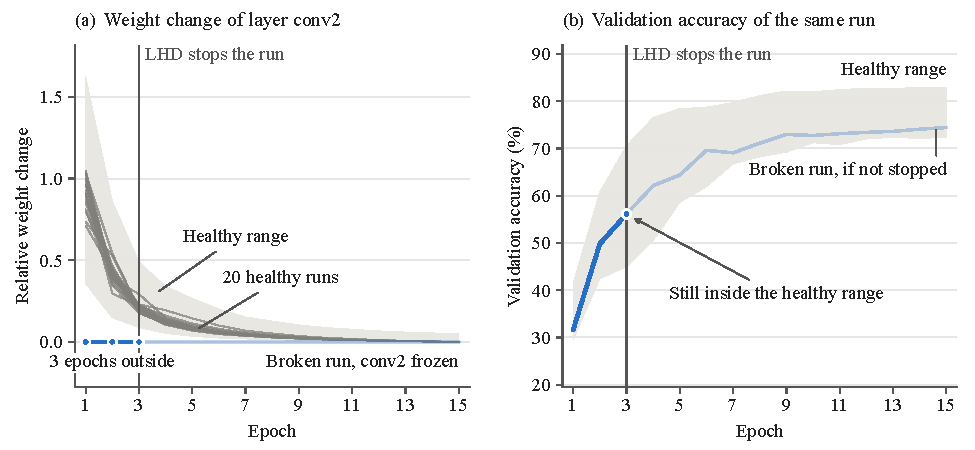
\includegraphics[width=\linewidth]{figures/how_lhd_works.pdf}
\caption{SOHAN WRITES THIS}
\label{fig:how_lhd_works}
\end{figure}

\section{Experimental Setup}
\label{sec:setup}

% BUDGET 0.5 page, including Table 2
% NUMBERS. Each \lhd macro prints the value next to it, and typing the value works too.
%   885                     \lhdRuns               runs in total  [results/tables/run_counts.csv]
%   60                      \lhdCalibrationRuns    calibration runs, all networks  [results/summary.json]
%   150                     \lhdFreshRuns          fresh healthy runs, all networks  [results/summary.json]
%   470                     \lhdBrokenRuns         broken runs with a frozen layer or dead units  [results/summary.json]
%   205                     \lhdOtherRuns          runs with the extra faults (third set)  [results/summary.json]
%   256, 128, 64            \lhdMlpWidths          hidden widths of the fully connected network  [experiments/models.py]
%   8, 16, 32               \lhdCnnFilters         filters in the CNN's three convolutions  [experiments/models.py]
%   64                      \lhdCnnDense           units in the CNN's dense layer  [experiments/models.py]
%   64                      \lhdTransformerWidth   transformer width  [experiments/models.py]
%   4                       \lhdTransformerHeads   transformer heads  [experiments/models.py]
%   2                       \lhdTransformerBlocks  transformer depth  [experiments/models.py]
%   256                     \lhdTransformerHidden  transformer hidden  [experiments/models.py]
%   0.001                   \lhdLearningRate       Adam learning rate  [experiments/train.py]
%   1                       \lhdThreads            CPU threads per run  [experiments/train.py]
%   0 to 19                 \lhdCalibrationSeeds   calibration seeds  [experiments/grid.py]
%   1000                    \lhdScoredSeedStart    first seed of scored runs  [experiments/grid.py]
%   10                      \lhdSeedsPerFault      seeds per fault condition  [experiments/grid.py]
%   10%, 25%, and 50%       \lhdDeadFractions      dead unit shares planted  [experiments/grid.py]
%   -1                      \lhdDeadBias           bias given to killed units  [experiments/train.py]
%   25%, 50%, 70%, and 80%  \lhdDeadChecks         fixed dead unit thresholds scored  [experiments/evaluate.py]
%   3                       \lhdPatience           patience p, epochs in a row  [experiments/evaluate.py]
%   b6bfb6a                 \lhdPlanCommit         commit with the run plan  [experiments/paper.py]
%   31 October 2026         \lhdPlanDate           date of that commit  [git log]
% FACTS
%   Adam with a cosine schedule, one CPU thread  [experiments/train.py]
%   A broken run and the fresh healthy run with the same seed differ only by the fault; that run is its twin, and the twin's final accuracy gives the fault's cost
%   Frozen layer: weights and bias put back after every optimizer step, the same failure as a layer left out of the optimizer; planted in every watched layer  [src/lhd/faults.py]
%   Dead units: incoming weights 0 and bias as above, so the ReLU output is 0 for every input; planted in every layer followed by a ReLU  [experiments/train.py]
%   Every run trained to the end, and LHD's alarm comes from replaying the saved signals  [src/lhd/replay.py]
%   Accuracy curve: fires when validation accuracy is below the lowest calibration value p epochs in a row, with no margin  [experiments/evaluate.py]
%   Zero update check: a layer's weights do not move in an epoch, like SageMaker's UnchangedTensor
%   Dead unit checks at the thresholds above: SageMaker DeadRelu 50%, DeepDiagnosis 70%, wandb-callbacks 80%, plus a 25% rule and any dead unit; all held to p epochs and counted only at the planted layer
%   Caught means the detector fired at or after the fault's onset; a false alarm is any alarm on a fresh healthy run; the gap is the accuracy curve's epoch minus LHD's, never counted as one past the end
SOHAN WRITES THIS
% TABLE shows each network's dataset, size, epochs, and runs, with a total row. The tabular is rebuilt from the data, so edit only the caption.
\begin{table}[t]
\centering
\small
\caption{SOHAN WRITES THIS}
\label{tab:networks}
\begin{tabular}{@{}llrrrrrr@{}}
\toprule
 & & & & & Fresh & Frozen & Other \\
Network & Dataset & Parameters & Epochs & Calibration & healthy & or dead & faults \\
\midrule
Fully connected & Fashion-MNIST & 242,762 & 20 & 20 & 50 & 130 & 55 \\
Transformer & Tiny Shakespeare & 112,577 & 15 & 20 & 50 & 170 & 85 \\
CNN & GTSRB & 41,659 & 15 & 20 & 50 & 170 & 65 \\
\midrule
Total & & & & 60 & 150 & 470 & 205 \\
\bottomrule
\end{tabular}

\end{table}

\section{Results}
\label{sec:results}
% BUDGET 2 pages for the four parts below, split as suggested under each heading

\subsection{LHD and the accuracy curve}
\label{sec:detection}

% BUDGET about 0.6 page, including Table 3
% NUMBERS. Each \lhd macro prints the value next to it, and typing the value works too.
%   411         \lhdCaught          broken runs LHD caught  [results/summary.json]
%   470         \lhdBrokenRuns      broken runs with a frozen layer or dead units  [results/summary.json]
%   87%         \lhdCaughtRate      share of broken runs LHD caught  [results/summary.json]
%   84 to 90%   \lhdCaughtInterval  95% Wilson interval of that share  [results/summary.json]
%   166         \lhdAccCaught       broken runs the accuracy curve caught  [results/summary.json]
%   35%         \lhdAccCaughtRate   share the accuracy curve caught  [results/summary.json]
%   3           \lhdMedianEpoch     median epoch of LHD's alarm  [results/summary.json]
%   6           \lhdAccMedianEpoch  median epoch of the accuracy curve's alarm  [results/summary.json]
%   61%         \lhdAccNever        runs LHD caught that the accuracy curve never caught  [results/summary.json]
%   66%         \lhdSilentShare     broken runs whose final accuracy ended inside the healthy range  [results/summary.json]
%   162         \lhdBothCaught      broken runs both LHD and the accuracy curve caught  [results/tables/runs.csv]
%   4.6         \lhdBothGap         mean epochs LHD was earlier on those runs  [results/tables/runs.csv]
%   3           \lhdBothMedian      median epochs LHD was earlier on those runs  [results/tables/runs.csv]
%   1           \lhdBothAccEarlier  of those runs, accuracy curve earlier  [results/tables/runs.csv]
%   26          \lhdBothTies        of those runs, same epoch  [results/tables/runs.csv]
%   30          \lhdSeedGroups      seed groups (network and seed)  [results/summary.json]
%   30          \lhdSeedGroupsLHD   seed groups whose mean gap favored LHD  [results/summary.json]
%   98.1%       \lhdLayerRight      caught runs where LHD named the planted layer  [results/summary.json]
%   403 of 411  \lhdLayerRightRuns  the same as runs  [results/summary.json]
%   96.8%       \lhdCauseRight      caught runs where LHD named the planted cause  [results/summary.json]
%   398 of 411  \lhdCauseRightRuns  the same as runs  [results/summary.json]
% FACTS
%   Per network values are in Table 3  [tables/headline.tex]
%   Epoch 3 is the earliest alarm possible for a fault planted at epoch 1 when p is 3
%   Figure A1 in the appendix shows the share flagged by each epoch
SOHAN WRITES THIS
% TABLE shows LHD next to the accuracy curve in each network. The tabular is rebuilt from the data, so edit only the caption.
\begin{table}[t]
\centering
\small
\caption{SOHAN WRITES THIS}
\label{tab:headline}
\begin{tabular}{@{}lrrrrrr@{}}
\toprule
 & \multicolumn{2}{c}{Fully connected} & \multicolumn{2}{c}{Transformer} & \multicolumn{2}{c}{CNN} \\
\cmidrule(lr){2-3} \cmidrule(lr){4-5} \cmidrule(lr){6-7}
 & LHD & Accuracy & LHD & Accuracy & LHD & Accuracy \\
\midrule
Broken runs caught & \textbf{84\%} & 26\% & \textbf{100\%} & 48\% & \textbf{78\%} & 29\% \\
Median epoch of the alarm & \textbf{3} & 17 & \textbf{3} & 5 & \textbf{3} & 7 \\
Healthy runs flagged & 1 of 50 & 1 of 50 & \textbf{0 of 50} & 6 of 50 & 2 of 50 & \textbf{0 of 50} \\
\bottomrule
\end{tabular}

\end{table}

\subsection{Faults that cost accuracy}
\label{sec:harm}

% BUDGET about 0.3 page
% NUMBERS. Each \lhd macro prints the value next to it, and typing the value works too.
%   223   \lhdHarmSmall        broken runs whose fault cost under 0.5 pts  [results/tables/harm.csv]
%   186   \lhdHarmSmallLHD     of those, LHD caught  [results/tables/harm.csv]
%   33    \lhdHarmSmallAcc     of those, the accuracy curve caught  [results/tables/harm.csv]
%   142   \lhdHarmMid          broken runs whose fault cost 0.5 to 2 pts  [results/tables/harm.csv]
%   131   \lhdHarmMidLHD       of those, LHD caught  [results/tables/harm.csv]
%   73    \lhdHarmMidAcc       of those, the accuracy curve caught  [results/tables/harm.csv]
%   105   \lhdHarmBig          broken runs whose fault cost 2 pts or more  [results/tables/harm.csv]
%   94    \lhdHarmBigLHD       of those, LHD caught  [results/tables/harm.csv]
%   60    \lhdHarmBigAcc       of those, the accuracy curve caught  [results/tables/harm.csv]
%   11.1  \lhdCnnFrozenDrop    mean accuracy points a frozen CNN layer cost against the twin  [results/tables/runs.csv]
%   3.1   \lhdCnnHalfDeadDrop  mean points half a CNN layer's units dead cost  [results/tables/runs.csv]
%   0.8   \lhdOtherMaxDrop     largest mean cost of any fault in the other two networks  [results/tables/runs.csv]
% FACTS
%   Cost is the final accuracy below the healthy twin with the same seed
%   Compare with your GTSRB model, where the frozen convolution cost 11 points
SOHAN WRITES THIS

\subsection{Dead units and fixed thresholds}
\label{sec:fixed}

% BUDGET about 0.8 page, including Figure 2
% NUMBERS. Each \lhd macro prints the value next to it, and typing the value works too.
%   200 of 200  \lhdZeroFrozenRuns      frozen layers the zero update check caught at the planted layer  [results/tables/detectors.csv]
%   200 of 200  \lhdZeroFrozenOneEpoch  the same check when one epoch is enough  [results/tables/detectors.csv]
%   1           \lhdZeroEpoch           median epoch of that one epoch check  [results/tables/detectors.csv]
%   3           \lhdLhdFrozenEpoch      median epoch of LHD's alarm on frozen layers  [results/tables/detectors.csv]
%   2           \lhdZeroLead            epochs the zero update check fires before LHD  [results/tables/detectors.csv]
%   0           \lhdZeroFlagged         Zero update check, healthy runs flagged (of 150)  [results/tables/detectors.csv]
%   97%         \lhdLhdFrozenRight      frozen layers LHD caught at the planted layer  [results/tables/detectors.csv]
%   78%         \lhdLhdDeadRight        dead unit faults LHD caught at the planted layer  [results/tables/detectors.csv]
%   78%         \lhdLhdDeadAny          dead unit faults LHD caught at any layer  [results/tables/detectors.csv]
%   3           \lhdFalseAlarms         fresh healthy runs LHD flagged  [results/summary.json]
%   71%         \lhdQuarterDead         25% dead rule, dead unit faults caught at the planted layer  [results/tables/detectors.csv]
%   51          \lhdQuarterFlagged      25% dead rule, healthy runs flagged (of 150)  [results/tables/detectors.csv]
%   40%         \lhdSageDead            SageMaker Debugger (50%), dead unit faults caught at the planted layer  [results/tables/detectors.csv]
%   22          \lhdSageFlagged         SageMaker Debugger (50%), healthy runs flagged (of 150)  [results/tables/detectors.csv]
%   4%          \lhdDeepDead            DeepDiagnosis (70%), dead unit faults caught at the planted layer  [results/tables/detectors.csv]
%   0           \lhdDeepFlagged         DeepDiagnosis (70%), healthy runs flagged (of 150)  [results/tables/detectors.csv]
%   0%          \lhdWandbDead           wandb-callbacks (80%), dead unit faults caught at the planted layer  [results/tables/detectors.csv]
%   0           \lhdWandbFlagged        wandb-callbacks (80%), healthy runs flagged (of 150)  [results/tables/detectors.csv]
%   74%         \lhdAnyDeadDead         Any dead unit (wandb-callbacks verbose), dead unit faults caught at the planted layer  [results/tables/detectors.csv]
%   100         \lhdAnyDeadFlagged      Any dead unit (wandb-callbacks verbose), healthy runs flagged (of 150)  [results/tables/detectors.csv]
%   36%         \lhdCnnDenseLow         fewest dead units in the CNN's fc1, calibration runs  [results/tables/signals.csv.gz]
%   70%         \lhdCnnDenseHigh        most dead units in the CNN's fc1, calibration runs  [results/tables/signals.csv.gz]
%   0%          \lhdTransformerDeadMax  most dead units in any transformer ReLU layer, calibration  [results/tables/signals.csv.gz]
% FACTS
%   Every fixed rule is held to p epochs and counted only when it names the planted layer; the full table is Table A1 in the appendix
%   A frozen layer's weight change is exactly 0, so a check for an exact 0 needs no range and no patience
SOHAN WRITES THIS
% FIGURE shows dead unit faults caught at the planted layer against healthy runs flagged, for LHD and each fixed rule
\begin{figure}[t]
\centering
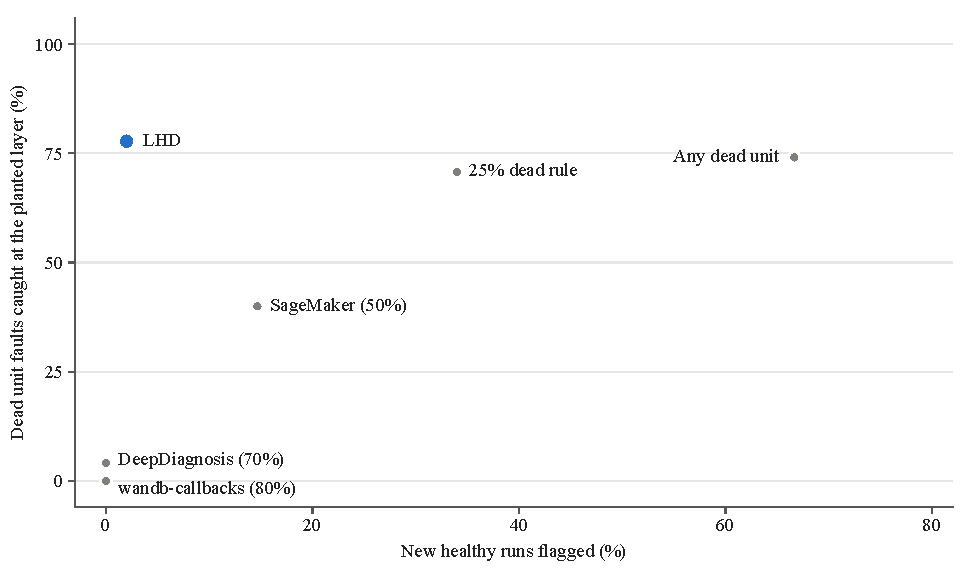
\includegraphics[width=\linewidth]{figures/detectors_tradeoff.pdf}
\caption{SOHAN WRITES THIS}
\label{fig:detectors_tradeoff}
\end{figure}

\subsection{False alarms}
\label{sec:alarms}

% BUDGET about 0.3 page
% NUMBERS. Each \lhd macro prints the value next to it, and typing the value works too.
%   3                     \lhdFalseAlarms            fresh healthy runs LHD flagged  [results/summary.json]
%   150                   \lhdHealthyRuns            fresh healthy runs scored  [results/summary.json]
%   2.0%                  \lhdFalseAlarmRate         LHD false alarm rate  [results/summary.json]
%   0.7 to 5.7%           \lhdFalseAlarmInterval     95% Wilson interval of that rate  [results/summary.json]
%   7                     \lhdAccFalseAlarms         fresh healthy runs the accuracy curve flagged  [results/summary.json]
%   2.3 to 9.3%           \lhdAccFalseAlarmInterval  95% Wilson interval of that rate  [results/summary.json]
%   mlp-fresh-none-s1046  \lhdAlarmARun              false alarm run  [results/tables/false_alarms.csv]
%   fc2                   \lhdAlarmALayer            layer it named  [results/tables/false_alarms.csv]
%   16                    \lhdAlarmAEpoch            epoch it fired  [results/tables/false_alarms.csv]
%   dead unit fraction    \lhdAlarmASignal           signal out of range  [results/tables/false_alarms.csv]
%   1.6%                  \lhdAlarmAValue            dead units in that layer at the alarm  [results/tables/signals.csv.gz]
%   3.9%                  \lhdAlarmAEdge             calibration lowest for that layer, so the alarm is below  [results/tables/signals.csv.gz]
%   cnn-fresh-none-s1015  \lhdAlarmBRun              false alarm run  [results/tables/false_alarms.csv]
%   conv2                 \lhdAlarmBLayer            layer it named  [results/tables/false_alarms.csv]
%   4                     \lhdAlarmBEpoch            epoch it fired  [results/tables/false_alarms.csv]
%   dead unit fraction    \lhdAlarmBSignal           signal out of range  [results/tables/false_alarms.csv]
%   6.2%                  \lhdAlarmBValue            dead units in that layer at the alarm  [results/tables/signals.csv.gz]
%   0.0%                  \lhdAlarmBEdge             calibration highest for that layer, so the alarm is above  [results/tables/signals.csv.gz]
%   cnn-fresh-none-s1028  \lhdAlarmCRun              false alarm run  [results/tables/false_alarms.csv]
%   conv2                 \lhdAlarmCLayer            layer it named  [results/tables/false_alarms.csv]
%   3                     \lhdAlarmCEpoch            epoch it fired  [results/tables/false_alarms.csv]
%   dead unit fraction    \lhdAlarmCSignal           signal out of range  [results/tables/false_alarms.csv]
%   6.2%                  \lhdAlarmCValue            dead units in that layer at the alarm  [results/tables/signals.csv.gz]
%   0.0%                  \lhdAlarmCEdge             calibration highest for that layer, so the alarm is above  [results/tables/signals.csv.gz]
%   0.05                  \lhdFloor                  floor f  [experiments/evaluate.py]
%   16                    \lhdSmallLayerUnits        units in the CNN's conv2  [experiments/models.py]
%   6.25%                 \lhdOneUnitShare           one dead unit in that layer  [experiments/models.py]
%   d3f5275               \lhdDraftCommit            commit of the earlier draft  [experiments/paper.py]
%   110                   \lhdDraftFresh             fresh healthy runs done at that draft  [experiments/paper.py]
%   3                     \lhdDraftAlarms            false alarms that draft reported  [experiments/paper.py]
%   40                    \lhdLaterFresh             fresh healthy runs finished after that draft  [results/tables/runs.csv]
%   0                     \lhdLaterAlarms            false alarms those later runs added  [results/summary.json]
% FACTS
%   When no calibration run has a dead unit in a layer, the top of its range is the floor, so one dead unit can cross it
%   An alarm for too few dead units points to no fault; checking only the top of the range would remove it
SOHAN WRITES THIS

\section{Limitations}
\label{sec:limits}

% BUDGET 0.5 page. Every item below must stay in.
% NUMBERS. Each \lhd macro prints the value next to it, and typing the value works too.
%   200 of 200              \lhdZeroFrozenOneEpoch  the same check when one epoch is enough  [results/tables/detectors.csv]
%   1                       \lhdZeroEpoch           median epoch of that one epoch check  [results/tables/detectors.csv]
%   2                       \lhdZeroLead            epochs the zero update check fires before LHD  [results/tables/detectors.csv]
%   78%                     \lhdLhdDeadRight        dead unit faults LHD caught at the planted layer  [results/tables/detectors.csv]
%   20                      \lhdCalibrationPerNet   calibration runs per network  [experiments/grid.py]
%   2                       \lhdCalARuns            calibration runs used to build the range  [results/tables/sweep_calibration.csv]
%   22%                     \lhdCalAWorst           highest mean false alarm rate over networks at that size  [results/tables/sweep_calibration.csv]
%   CNN                     \lhdCalANet             network with that rate  [results/tables/sweep_calibration.csv]
%   3                       \lhdCalBRuns            calibration runs used to build the range  [results/tables/sweep_calibration.csv]
%   15%                     \lhdCalBWorst           highest mean false alarm rate over networks at that size  [results/tables/sweep_calibration.csv]
%   CNN                     \lhdCalBNet             network with that rate  [results/tables/sweep_calibration.csv]
%   5                       \lhdCalCRuns            calibration runs used to build the range  [results/tables/sweep_calibration.csv]
%   11%                     \lhdCalCWorst           highest mean false alarm rate over networks at that size  [results/tables/sweep_calibration.csv]
%   fully connected network  \lhdCalCNet             network with that rate  [results/tables/sweep_calibration.csv]
%   10                      \lhdCalDRuns            calibration runs used to build the range  [results/tables/sweep_calibration.csv]
%   5%                      \lhdCalDWorst           highest mean false alarm rate over networks at that size  [results/tables/sweep_calibration.csv]
%   fully connected network  \lhdCalDNet             network with that rate  [results/tables/sweep_calibration.csv]
%   15                      \lhdCalERuns            calibration runs used to build the range  [results/tables/sweep_calibration.csv]
%   4%                      \lhdCalEWorst           highest mean false alarm rate over networks at that size  [results/tables/sweep_calibration.csv]
%   CNN                     \lhdCalENet             network with that rate  [results/tables/sweep_calibration.csv]
%   20                      \lhdCalFRuns            calibration runs used to build the range  [results/tables/sweep_calibration.csv]
%   4%                      \lhdCalFWorst           highest mean false alarm rate over networks at that size  [results/tables/sweep_calibration.csv]
%   CNN                     \lhdCalFNet             network with that rate  [results/tables/sweep_calibration.csv]
%   36%                     \lhdCnnDenseLow         fewest dead units in the CNN's fc1, calibration runs  [results/tables/signals.csv.gz]
%   70%                     \lhdCnnDenseHigh        most dead units in the CNN's fc1, calibration runs  [results/tables/signals.csv.gz]
%   0 of 10                 \lhdCnnDenseACaught     CNN fc1 runs with 10% dead units that LHD caught  [results/tables/per_layer.csv]
%   0 of 10                 \lhdCnnDenseBCaught     CNN fc1 runs with 25% dead units that LHD caught  [results/tables/per_layer.csv]
%   1 of 10                 \lhdCnnDenseCCaught     CNN fc1 runs with 50% dead units that LHD caught  [results/tables/per_layer.csv]
%   223                     \lhdHarmSmall           broken runs whose fault cost under 0.5 pts  [results/tables/harm.csv]
%   470                     \lhdBrokenRuns          broken runs with a frozen layer or dead units  [results/summary.json]
%   35                      \lhdVanishingFired      runs named vanishing gradient, extra faults only  [results/summary.json]
%   5                       \lhdRunawayFired        runs named runaway weights, extra faults only  [results/summary.json]
%   0                       \lhdDivergenceFired     runs where the divergence rule fired, all faults  [results/summary.json]
%   0.05                    \lhdFloor               floor f  [experiments/evaluate.py]
%   16                      \lhdSmallLayerUnits     units in the CNN's conv2  [experiments/models.py]
%   6.25%                   \lhdOneUnitShare        one dead unit in that layer  [experiments/models.py]
%   15 to 20                \lhdEpochRange          epochs per run  [experiments/train.py]
%   37%                     \lhdTransformerAcc      mean final next character accuracy of fresh transformer runs  [results/tables/runs.csv]
%   242,762                 \lhdMlpParams           parameters, fully connected network  [results/tables/networks.csv]
%   41,659                  \lhdCnnParams           parameters, CNN  [results/tables/networks.csv]
%   112,577                 \lhdTransformerParams   parameters, transformer  [results/tables/networks.csv]
%   1                       \lhdThreads             CPU threads per run  [experiments/train.py]
%   60                      \lhdFreshThirdSet       fresh healthy runs in the third set  [results/tables/runs.csv]
%   205                     \lhdOtherRuns           runs with the extra faults (third set)  [results/summary.json]
%   5                       \lhdWrongCauseRuns      right layer but wrong cause  [results/tables/runs.csv]
%   a frozen b1.qkv in the transformer called vanishing gradient (5)  \lhdWrongCauseList      those runs  [results/tables/runs.csv]
% FACTS
%   1. The zero update check catches frozen layers 2 epochs sooner (200 of 200 at epoch 1); LHD's advantage is dead units
%   2. Faults were planted to show up in the signals LHD measures; they are not real bugs
%   3. Calibration needs 10 to 20 healthy runs of the same network and assumes they are healthy; this costs more than LHD saves for a model trained once. The study used 20 per network, and the Cal numbers above show the false alarms at each size
%   4. LHD misses dead units where healthy runs already lose many units (the CNN's dense layer, 36% to 70% dead in healthy runs)
%   5. 223 of 470 planted faults cost less than half a point of accuracy
%   6. Only the frozen layer and dead unit rules were tested in the main study; the divergence rule never fired (0 runs). In the main study the vanishing gradient rule fired only as a wrong cause, a frozen b1.qkv in the transformer called vanishing gradient (5)
%   7. The 0.05 floor is too low for small layers; one dead unit of 16 is 6.25%
%   8. Small networks, laptop CPU, 15 to 20 epochs; the transformer reaches about 37% accuracy; no GPU, large models, or other optimizers
%   9. The third set of runs (60 healthy runs and the extra faults) was trained after the main results
SOHAN WRITES THIS

\section{Conclusion}
\label{sec:conclusion}

% BUDGET 3 sentences
% NUMBERS. Each \lhd macro prints the value next to it, and typing the value works too.
%   885    \lhdRuns          runs in total  [results/tables/run_counts.csv]
%   87%    \lhdCaughtRate    share of broken runs LHD caught  [results/summary.json]
%   98.1%  \lhdLayerRight    caught runs where LHD named the planted layer  [results/summary.json]
%   3      \lhdFalseAlarms   fresh healthy runs LHD flagged  [results/summary.json]
%   150    \lhdHealthyRuns   fresh healthy runs scored  [results/summary.json]
%   78%    \lhdLhdDeadRight  dead unit faults LHD caught at the planted layer  [results/tables/detectors.csv]
SOHAN WRITES THIS

% MAIN TEXT ENDS HERE. Everything above must fit in 6 pages.
\FloatBarrier

\section*{Use of generative AI}
\label{sec:ai}

% BUDGET not counted
% FACTS
%   The long paper's statement, for reference  [paper/lhd.tex]
%   The author came up with the idea, designed the study in an earlier proposal, and wrote the core LHD library (signals, detector, and diagnosis), with Claude, made by Anthropic, providing function outlines and docstrings. Claude wrote the experiment scripts that trained and scored the networks, ran the training runs, wrote the analysis and figure code, and drafted parts of this paper, including the results and related work. The author directed the study, decided what to test and change, and is responsible for all of its content.
SOHAN WRITES THIS

\section*{Code and data}
\label{sec:code}

% BUDGET not counted
% NUMBERS. Each \lhd macro prints the value next to it, and typing the value works too.
%   b6bfb6a  \lhdPlanCommit      commit with the run plan  [experiments/paper.py]
%   d3f5275  \lhdDraftCommit     commit of the earlier draft  [experiments/paper.py]
%   e83806f  \lhdSettingsCommit  commit that fixed m, f, and p  [experiments/paper.py]
% FACTS
%   Repository https://github.com/sohan-bhat/lhd
%   The long version is tagged v0-long
SOHAN WRITES THIS

\begin{thebibliography}{99}

\bibitem[Amazon Web Services(n.d.a)]{aws_rules}
Amazon Web Services (n.d.a).
\newblock List of Debugger built-in rules.
\newblock Amazon SageMaker AI Developer Guide.
\newblock \url{https://docs.aws.amazon.com/sagemaker/latest/dg/debugger-built-in-rules.html}

\bibitem[Amazon Web Services(n.d.b)]{aws_actions}
Amazon Web Services (n.d.b).
\newblock Use Debugger built-in actions for rules.
\newblock Amazon SageMaker AI Developer Guide.
\newblock \url{https://docs.aws.amazon.com/sagemaker/latest/dg/debugger-built-in-actions.html}

\bibitem[Biewald(2020)]{biewald2020}
Biewald, L. (2020).
\newblock Experiment tracking with Weights and Biases.
\newblock Software available from wandb.com.
\newblock \url{https://www.wandb.com/}

\bibitem[Chwilczy\'nski et~al.(2024)]{chwilczynski2024}
Chwilczy\'nski, S., Tr\k{e}bacz, K., Cyganik, K., Ma\l{}ecki, M., and Brzezinski, D. (2024).
\newblock ART: Actually Robust Training.
\newblock In \emph{Machine Learning and Knowledge Discovery in Databases. Research Track and Demo Track (ECML PKDD 2024)}, Lecture Notes in Computer Science, vol.~14948, pp.~374--378. Springer, Cham.
\newblock \url{https://doi.org/10.1007/978-3-031-70371-3_23}. Preprint: arXiv:2408.16285.

\bibitem[CS231n(n.d.)]{cs231n}
CS231n (n.d.).
\newblock Neural networks part 3: Learning and evaluation.
\newblock Course notes for CS231n, Stanford University.
\newblock \url{https://cs231n.github.io/neural-networks-3/}

\bibitem[Groeger(n.d.)]{groeger_wandbcallbacks}
Groeger, F. (n.d.).
\newblock wandb-callbacks: Additional callbacks for Weights \& Biases.
\newblock GitHub repository.
\newblock \url{https://github.com/FabianGroeger96/wandb-callbacks}

\bibitem[Karpathy(2019)]{karpathy2019}
Karpathy, A. (2019).
\newblock A recipe for training neural networks.
\newblock Blog post, April 25, 2019.
\newblock \url{https://karpathy.github.io/2019/04/25/recipe/}

\bibitem[Stallkamp et~al.(2012)]{stallkamp2012}
Stallkamp, J., Schlipsing, M., Salmen, J., and Igel, C. (2012).
\newblock Man vs.\ computer: Benchmarking machine learning algorithms for traffic sign recognition.
\newblock \emph{Neural Networks}, 32:323--332.
\newblock \url{https://doi.org/10.1016/j.neunet.2012.02.016}

\bibitem[Wardat et~al.(2022)]{wardat2022}
Wardat, M., Cruz, B.~D., Le, W., and Rajan, H. (2022).
\newblock DeepDiagnosis: Automatically diagnosing faults and recommending actionable fixes in deep learning programs.
\newblock In \emph{Proceedings of the 44th International Conference on Software Engineering (ICSE 2022)}, pp.~561--572. ACM, New York.
\newblock \url{https://doi.org/10.1145/3510003.3510071}. Preprint: arXiv:2112.04036.

\bibitem[Zhang et~al.(2021)]{zhang2021}
Zhang, X., Zhai, J., Ma, S., and Shen, C. (2021).
\newblock AUTOTRAINER: An automatic DNN training problem detection and repair system.
\newblock In \emph{2021 IEEE/ACM 43rd International Conference on Software Engineering (ICSE)}, pp.~359--371. IEEE.
\newblock \url{https://doi.org/10.1109/ICSE43902.2021.00043}

\end{thebibliography}


\clearpage
\appendix
\setcounter{figure}{0}
\setcounter{table}{0}
\renewcommand{\thefigure}{A\arabic{figure}}
\renewcommand{\thetable}{A\arabic{table}}

\section{Networks and runs in detail}
\label{app:runs}

% BUDGET not counted
% NUMBERS. Each \lhd macro prints the value next to it, and typing the value works too.
%   256, 128, 64     \lhdMlpWidths          hidden widths of the fully connected network  [experiments/models.py]
%   8, 16, 32        \lhdCnnFilters         filters in the CNN's three convolutions  [experiments/models.py]
%   64               \lhdCnnDense           units in the CNN's dense layer  [experiments/models.py]
%   64               \lhdTransformerWidth   transformer width  [experiments/models.py]
%   4                \lhdTransformerHeads   transformer heads  [experiments/models.py]
%   2                \lhdTransformerBlocks  transformer depth  [experiments/models.py]
%   256              \lhdTransformerHidden  transformer hidden  [experiments/models.py]
%   4,000            \lhdCnnValImages       CNN validation images  [experiments/train.py]
%   512              \lhdTextWindows        transformer validation windows  [experiments/data.py]
%   64               \lhdTextContext        characters per window  [experiments/train.py]
%   10%              \lhdTextHeldOut        share of the text held out for validation  [experiments/data.py]
%   0 to 19          \lhdCalibrationSeeds   calibration seeds  [experiments/grid.py]
%   1000             \lhdScoredSeedStart    first seed of scored runs  [experiments/grid.py]
%   10               \lhdSeedsPerFault      seeds per fault condition  [experiments/grid.py]
%   7919             \lhdUnitSeedOffset     added to the run's seed to pick the killed units  [experiments/train.py]
%   -1               \lhdDeadBias           bias given to killed units  [experiments/train.py]
%   90               \lhdFreshFirstSet      fresh healthy runs in the first set  [results/tables/runs.csv]
%   60               \lhdFreshThirdSet      fresh healthy runs in the third set  [results/tables/runs.csv]
%   b6bfb6a          \lhdPlanCommit         commit with the run plan  [experiments/paper.py]
%   31 October 2026  \lhdPlanDate           date of that commit  [git log]
% FACTS
%   fully connected network: watched layers fc1, fc2, fc3, fc4; ReLU layers where units can die fc1, fc2, fc3  [experiments/models.py]
%   transformer: watched layers tok, pos, b0.qkv, b0.proj, b0.ff1, b0.ff2, b1.qkv, b1.proj, b1.ff1, b1.ff2, head; ReLU layers where units can die b0.ff1, b1.ff1  [experiments/models.py]
%   CNN: watched layers conv1, conv2, conv3, fc1, fc2; ReLU layers where units can die conv1, conv2, conv3, fc1  [experiments/models.py]
%   Killed units are drawn without replacement, their number is the share times the layer's width rounded with at least one unit, and Adam's running averages for them are cleared  [experiments/train.py]
%   Statistics: one sided Wilcoxon signed rank test on the gap averaged within each seed and within each fault condition, a bootstrap with 10,000 draws that resamples whole seeds, and Wilson score intervals for rates  [experiments/evaluate.py]
SOHAN WRITES THIS

\section{Detection over time}
\label{app:time}

% BUDGET not counted
% NUMBERS. Each \lhd macro prints the value next to it, and typing the value works too.
%   84%   \lhdTimeMlpLhd          broken runs LHD flagged by the end, fully connected network  [experiments/paper_figures.py]
%   26%   \lhdTimeMlpAcc          broken runs the accuracy curve flagged by the end, fully connected network  [experiments/paper_figures.py]
%   100%  \lhdTimeTransformerLhd  broken runs LHD flagged by the end, transformer  [experiments/paper_figures.py]
%   48%   \lhdTimeTransformerAcc  broken runs the accuracy curve flagged by the end, transformer  [experiments/paper_figures.py]
%   78%   \lhdTimeCnnLhd          broken runs LHD flagged by the end, CNN  [experiments/paper_figures.py]
%   29%   \lhdTimeCnnAcc          broken runs the accuracy curve flagged by the end, CNN  [experiments/paper_figures.py]
SOHAN WRITES THIS
% FIGURE shows the share of broken runs flagged by each epoch, LHD against the accuracy curve, one panel per network
\begin{figure}[t]
\centering
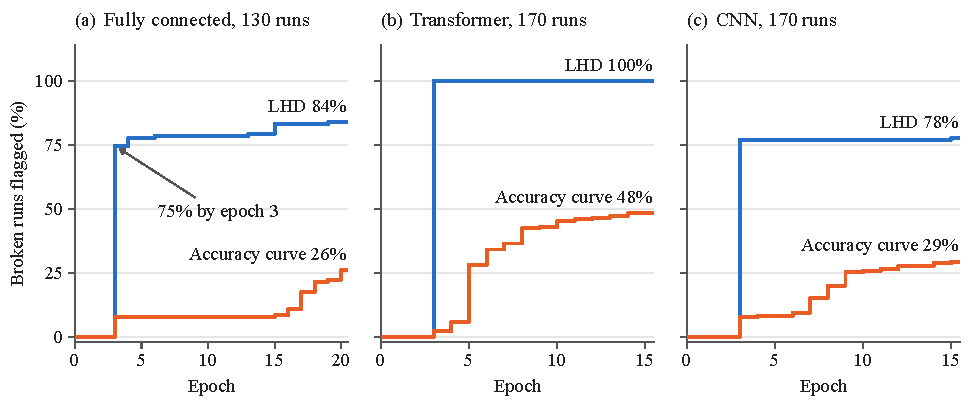
\includegraphics[width=\linewidth]{figures/detection_over_time.pdf}
\caption{SOHAN WRITES THIS}
\label{fig:detection_over_time}
\end{figure}

\section{Every detector}
\label{app:detectors}

% BUDGET not counted
% NUMBERS. Each \lhd macro prints the value next to it, and typing the value works too.
%   0           \lhdPatienceAlarmChange  largest change in false alarms between one and three epochs, fixed rules  [results/tables/detectors.csv]
%   2           \lhdPatienceDeadChange   largest drop in dead unit catches between one and three epochs  [results/tables/detectors.csv]
%   26          \lhdSageAnyTen           50% rule catches of 10% dead units at any layer  [results/tables/detectors.csv]
%   8           \lhdSageRightTen         50% rule catches of 10% dead units at the planted layer  [results/tables/detectors.csv]
%   25          \lhdSageAnyTwentyFive    50% rule catches of 25% dead units at any layer  [results/tables/detectors.csv]
%   10          \lhdSageRightTwentyFive  50% rule catches of 25% dead units at the planted layer  [results/tables/detectors.csv]
%   291 of 470  \lhdAccOneCaught         Accuracy curve, 1 epoch below healthy, broken runs caught  [results/tables/detectors.csv]
%   44 of 150   \lhdAccOneFlagged        Accuracy curve, 1 epoch below healthy, healthy runs flagged  [results/tables/detectors.csv]
%   143 of 470  \lhdLossCaught           Loss curve, 3 epochs above healthy, broken runs caught  [results/tables/detectors.csv]
%   9 of 150    \lhdLossFlagged          Loss curve, 3 epochs above healthy, healthy runs flagged  [results/tables/detectors.csv]
% FACTS
%   Requiring three epochs instead of one changed little, since a layer's dead unit fraction rarely drops back once it crosses a threshold
%   Counted at any layer, the 50% rule caught more runs with 10% dead units than with 25%, because it fired on units that died on their own in other layers
SOHAN WRITES THIS
% TABLE shows every detector held to three epochs, frozen layers and dead units caught at the planted layer, and healthy runs flagged. The tabular is rebuilt from the data, so edit only the caption.
\begin{table}[t]
\centering
\small
\caption{SOHAN WRITES THIS}
\label{tab:detectors}
\begin{tabular}{@{}lrrr@{}}
\toprule
 & \multicolumn{2}{c}{Caught at the planted layer} & \\
\cmidrule(lr){2-3}
Detector & Frozen layers & Dead units & Healthy runs flagged \\
\midrule
LHD & 97\% & \textbf{78\%} & 3 of 150 \\
Zero update check & \textbf{100\%} & 0\% & 0 of 150 \\
25\% dead rule & 0\% & 71\% & 51 of 150 \\
SageMaker Debugger (50\%) & 0\% & 40\% & 22 of 150 \\
DeepDiagnosis (70\%) & 0\% & 4\% & 0 of 150 \\
wandb-callbacks (80\%) & 0\% & 0\% & 0 of 150 \\
Any dead unit (wandb-callbacks verbose) & 2\% & 74\% & 100 of 150 \\
\bottomrule
\end{tabular}

\end{table}

\section{Each layer and how many units must die}
\label{app:layers}

% BUDGET not counted
% NUMBERS. Each \lhd macro prints the value next to it, and typing the value works too.
%   57%                     \lhdDoseALhd        LHD catches with 10% dead units  [results/tables/detectors.csv]
%   7%                      \lhdDoseAAcc        accuracy curve catches with 10% dead units  [results/tables/detectors.csv]
%   88%                     \lhdDoseBLhd        LHD catches with 25% dead units  [results/tables/detectors.csv]
%   9%                      \lhdDoseBAcc        accuracy curve catches with 25% dead units  [results/tables/detectors.csv]
%   90%                     \lhdDoseCLhd        LHD catches with 50% dead units  [results/tables/detectors.csv]
%   29%                     \lhdDoseCAcc        accuracy curve catches with 50% dead units  [results/tables/detectors.csv]
%   CNN conv3 at 10% (1 of 10); CNN fc1 at 10% (0 of 10); CNN fc1 at 25% (0 of 10); CNN fc1 at 50% (1 of 10); fully connected network fc2 at 10% (0 of 10); fully connected network fc3 at 10% (0 of 10); fully connected network fc3 at 25% (9 of 10)  \lhdDoseMisses      every layer and share where LHD missed some dead unit runs  [results/tables/per_layer.csv]
%   8                       \lhdWrongLayerRuns  caught runs where LHD named another layer  [results/tables/wrong_layers.csv]
%   50% dead units in fc1 in the CNN named fc2 (1); a frozen conv2 in the CNN named conv1 (1); a frozen conv3 in the CNN named conv2 (1); a frozen fc1 in the CNN named conv1 (1); a frozen fc1 in the CNN named conv2 (1); a frozen fc1 in the CNN named conv3 (3)  \lhdWrongLayerList  those runs  [results/tables/wrong_layers.csv]
%   5                       \lhdWrongCauseRuns  right layer but wrong cause  [results/tables/runs.csv]
%   a frozen b1.qkv in the transformer called vanishing gradient (5)  \lhdWrongCauseList  those runs  [results/tables/runs.csv]
% FACTS
%   In each wrong layer run, the layer LHD named had its own signal out of range
%   A frozen attention projection also lowers the gradient that reaches it, so its pattern can match a vanishing gradient
SOHAN WRITES THIS
% FIGURE shows for every layer and fault, the share of broken runs where LHD caught the fault and named both the planted layer and the right cause
\begin{figure}[t]
\centering
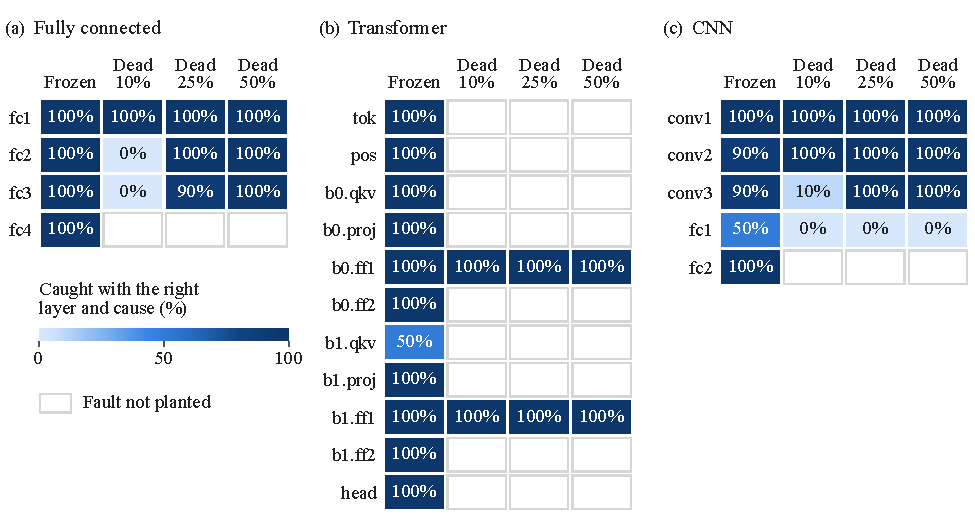
\includegraphics[width=\linewidth]{figures/per_layer.pdf}
\caption{SOHAN WRITES THIS}
\label{fig:per_layer}
\end{figure}

\section{What each signal adds}
\label{app:ablation}

% BUDGET not counted
% NUMBERS. Each \lhd macro prints the value next to it, and typing the value works too.
%   87%  \lhdAblationAllFourCaught   broken runs caught, all four  [results/tables/ablation.csv]
%   85%  \lhdAblationAllFourBoth     right layer and cause, all four  [results/tables/ablation.csv]
%   43%  \lhdAblationNoDeadCaught    broken runs caught, without dead unit fraction  [results/tables/ablation.csv]
%   41%  \lhdAblationNoDeadBoth      right layer and cause, without dead unit fraction  [results/tables/ablation.csv]
%   70%  \lhdAblationNoChangeCaught  broken runs caught, without weight change  [results/tables/ablation.csv]
%   45%  \lhdAblationNoChangeBoth    right layer and cause, without weight change  [results/tables/ablation.csv]
% FACTS
%   None of the planted faults was designed to move the weight norm or the gradient norm
SOHAN WRITES THIS
% TABLE shows the same runs replayed with each signal removed or used alone. The tabular is rebuilt from the data, so edit only the caption.
\begin{table}[t]
\centering
\small
\caption{SOHAN WRITES THIS}
\label{tab:ablation}
\begin{tabular}{@{}lrrrr@{}}
\toprule
Signals used & \multicolumn{2}{c}{Broken runs caught} & \multicolumn{2}{c}{Right layer and cause} \\
\cmidrule(lr){2-3} \cmidrule(l){4-5}
 & Rate & Change & Rate & Change \\
\midrule
All four & 87\% & & 85\% & \\
\midrule
Without weight change & 70\% & $-$18 & 45\% & $-$40 \\
Without weight norm & 87\% & same & 85\% & same \\
Without grad norm & 87\% & same & 86\% & +1 \\
Without dead unit fraction & 43\% & $-$45 & 41\% & $-$44 \\
\midrule
Only weight change & 43\% & $-$45 & 43\% & $-$42 \\
Only weight norm & 10\% & $-$77 & 0\% & $-$85 \\
Only grad norm & 25\% & $-$63 & 0\% & $-$85 \\
Only dead unit fraction & 52\% & $-$36 & 45\% & $-$40 \\
\bottomrule
\end{tabular}

\end{table}

\section{Margin and calibration size}
\label{app:settings}

% BUDGET not counted
% NUMBERS. Each \lhd macro prints the value next to it, and typing the value works too.
%   0.5                     \lhdMargin         margin m  [experiments/evaluate.py]
%   71%                     \lhdEdgeFlagged    healthy runs flagged with no margin  [results/tables/sweep_settings.csv]
%   98%                     \lhdEdgeCaught     broken runs caught with no margin  [results/tables/sweep_settings.csv]
%   2%                      \lhdMarginFlagged  healthy runs flagged with the margin used  [results/tables/sweep_settings.csv]
%   87%                     \lhdMarginCaught   broken runs caught with the margin used  [results/tables/sweep_settings.csv]
%   2                       \lhdCalARuns       calibration runs used to build the range  [results/tables/sweep_calibration.csv]
%   22%                     \lhdCalAWorst      highest mean false alarm rate over networks at that size  [results/tables/sweep_calibration.csv]
%   CNN                     \lhdCalANet        network with that rate  [results/tables/sweep_calibration.csv]
%   3                       \lhdCalBRuns       calibration runs used to build the range  [results/tables/sweep_calibration.csv]
%   15%                     \lhdCalBWorst      highest mean false alarm rate over networks at that size  [results/tables/sweep_calibration.csv]
%   CNN                     \lhdCalBNet        network with that rate  [results/tables/sweep_calibration.csv]
%   5                       \lhdCalCRuns       calibration runs used to build the range  [results/tables/sweep_calibration.csv]
%   11%                     \lhdCalCWorst      highest mean false alarm rate over networks at that size  [results/tables/sweep_calibration.csv]
%   fully connected network  \lhdCalCNet        network with that rate  [results/tables/sweep_calibration.csv]
%   10                      \lhdCalDRuns       calibration runs used to build the range  [results/tables/sweep_calibration.csv]
%   5%                      \lhdCalDWorst      highest mean false alarm rate over networks at that size  [results/tables/sweep_calibration.csv]
%   fully connected network  \lhdCalDNet        network with that rate  [results/tables/sweep_calibration.csv]
%   15                      \lhdCalERuns       calibration runs used to build the range  [results/tables/sweep_calibration.csv]
%   4%                      \lhdCalEWorst      highest mean false alarm rate over networks at that size  [results/tables/sweep_calibration.csv]
%   CNN                     \lhdCalENet        network with that rate  [results/tables/sweep_calibration.csv]
%   20                      \lhdCalFRuns       calibration runs used to build the range  [results/tables/sweep_calibration.csv]
%   4%                      \lhdCalFWorst      highest mean false alarm rate over networks at that size  [results/tables/sweep_calibration.csv]
%   CNN                     \lhdCalFNet        network with that rate  [results/tables/sweep_calibration.csv]
% FACTS
%   These checks replay the same saved runs after the main results; the settings were fixed before them  [experiments/sweep.py]
SOHAN WRITES THIS

\section{Cost}
\label{app:cost}

% BUDGET not counted
% NUMBERS. Each \lhd macro prints the value next to it, and typing the value works too.
%   11.6%  \lhdMlpOverhead          training time LHD added, fully connected network  [results/summary.json]
%   5.9%   \lhdTransformerOverhead  training time LHD added, transformer  [results/summary.json]
%   2.2%   \lhdCnnOverhead          training time LHD added, CNN  [results/summary.json]
%   70%    \lhdComputeSaved         mean training saved by stopping each broken run at LHD's alarm  [results/summary.json]
%   107    \lhdTrainingHours        CPU hours for all runs  [results/tables/compute.csv]
% FACTS
%   Measured on fresh healthy runs on one CPU thread; most of the overhead is the gradient norm, read after every batch, and the probe batch, run once per epoch
SOHAN WRITES THIS

\section{Faults beyond frozen layers and dead units}
\label{app:extra}

% BUDGET not counted
% NUMBERS. Each \lhd macro prints the value next to it, and typing the value works too.
%   6                       \lhdLateOnset         epoch the late faults and learning rate jumps start  [experiments/grid.py]
%   100                     \lhdLateFrozenRuns    runs, latefrozen  [results/summary.json]
%   100                     \lhdLateFrozenCaught  LHD caught, latefrozen  [results/summary.json]
%   100                     \lhdLateFrozenBoth    LHD named layer and cause, latefrozen  [results/tables/runs.csv]
%   20                      \lhdLateFrozenAcc     accuracy curve caught, latefrozen  [results/summary.json]
%   a frozen layer (100)    \lhdLateFrozenCauses  causes LHD named, latefrozen  [results/summary.json]
%   45                      \lhdLateDeadRuns      runs, latedead50  [results/summary.json]
%   40                      \lhdLateDeadCaught    LHD caught, latedead50  [results/summary.json]
%   40                      \lhdLateDeadBoth      LHD named layer and cause, latedead50  [results/tables/runs.csv]
%   7                       \lhdLateDeadAcc       accuracy curve caught, latedead50  [results/summary.json]
%   dead units (40)         \lhdLateDeadCauses    causes LHD named, latedead50  [results/summary.json]
%   30                      \lhdCutRuns           runs, detach  [results/summary.json]
%   30                      \lhdCutCaught         LHD caught, detach  [results/summary.json]
%   30                      \lhdCutBoth           LHD named layer and cause, detach  [results/tables/runs.csv]
%   30                      \lhdCutAcc            accuracy curve caught, detach  [results/summary.json]
%   a vanishing gradient (30)  \lhdCutCauses         causes LHD named, detach  [results/summary.json]
%   15                      \lhdLrTenRuns         runs, lr10  [results/summary.json]
%   15                      \lhdLrTenCaught       LHD caught, lr10  [results/summary.json]
%   0                       \lhdLrTenBoth         LHD named layer and cause, lr10  [results/tables/runs.csv]
%   5                       \lhdLrTenAcc          accuracy curve caught, lr10  [results/summary.json]
%   an unrecognized pattern (9); dead units (6)  \lhdLrTenCauses       causes LHD named, lr10  [results/summary.json]
%   15                      \lhdLrHundredRuns     runs, lr100  [results/summary.json]
%   15                      \lhdLrHundredCaught   LHD caught, lr100  [results/summary.json]
%   0                       \lhdLrHundredBoth     LHD named layer and cause, lr100  [results/tables/runs.csv]
%   15                      \lhdLrHundredAcc      accuracy curve caught, lr100  [results/summary.json]
%   dead units (5); runaway weights (5); a vanishing gradient (5)  \lhdLrHundredCauses   causes LHD named, lr100  [results/summary.json]
%   30 of 30                \lhdCutZero           gradient cuts the zero update check caught before the cut  [results/tables/detectors.csv]
%   37 of 45                \lhdLateDeadSage      late half dead runs the 50% rule caught at the planted layer  [results/tables/detectors.csv]
%   0.00075                 \lhdLrNormal          learning rate at epoch 6 in the 15 epoch networks  [experiments/train.py]
%   0.0075                  \lhdLrTimesTen        the same after a tenfold jump  [experiments/train.py]
%   0.075                   \lhdLrTimesHundred    the same after a hundredfold jump  [experiments/train.py]
%   6                       \lhdLateZeroEpoch     zero update check epoch on late frozen layers  [results/tables/detectors.csv]
%   100 of 100              \lhdLateZeroTies      late frozen runs where the three epoch check fired with LHD  [results/tables/detectors.csv]
%   30 of 30                \lhdCutZero           gradient cuts the zero update check caught before the cut  [results/tables/detectors.csv]
%   37 of 45                \lhdLateDeadSage      late half dead runs the 50% rule caught at the planted layer  [results/tables/detectors.csv]
%   22                      \lhdSageFlagged       SageMaker Debugger (50%), healthy runs flagged (of 150)  [results/tables/detectors.csv]
%   0                       \lhdDivergenceFired   runs where the divergence rule fired, all faults  [results/summary.json]
% FACTS
%   Late faults are the main faults started at the epoch above instead of epoch 1
%   A gradient cut detaches one layer's input from the first epoch, so no gradient reaches the layers before it  [experiments/grid.py DETACH_CUTS]
%   A learning rate jump multiplies Adam's rate at the start of that epoch, and the cosine schedule keeps shrinking it from the raised value
%   This third set was trained after the main results were in
SOHAN WRITES THIS
% TABLE shows each extra fault, caught by LHD, the accuracy curve, the zero update check, and the 50% rule, with healthy runs flagged. The tabular is rebuilt from the data, so edit only the caption.
\begin{table}[t]
\centering
\small
\caption{SOHAN WRITES THIS}
\label{tab:extra}
\begin{tabular}{@{}lrrrrr@{}}
\toprule
 & & & Accuracy & Zero update & 50\% dead \\
Fault & Runs & LHD & curve & check & rule \\
\midrule
Frozen layer at epoch 6 & 100 & 100\% & 20\% & 100\% & 0\% \\
50\% dead units at epoch 6 & 45 & \textbf{89\%} & 16\% & 0\% & 82\% \\
Gradient cut & 30 & 100\% & 100\% & 100\% & 0\% \\
Learning rate $\times 10$ at epoch 6 & 15 & \textbf{100\%} & 33\% & 0\% & 0\% \\
Learning rate $\times 100$ at epoch 6 & 15 & 100\% & 100\% & 67\% & 60\% \\
\midrule
Healthy runs flagged & 150 & 3 & 7 & \textbf{0} & 22 \\
\bottomrule
\end{tabular}

\end{table}

\section{Statistics for each seed and condition}
\label{app:stats}

% BUDGET not counted
% NUMBERS. Each \lhd macro prints the value next to it, and typing the value works too.
%   30                \lhdSeedGroups         seed groups (network and seed)  [results/summary.json]
%   30                \lhdSeedGroupsLHD      seed groups whose mean gap favored LHD  [results/summary.json]
%   p = 9.3 x 10^-10  \lhdSeedP              one sided Wilcoxon over seed groups  [results/summary.json]
%   47                \lhdConditions         fault conditions (network, fault, layer)  [results/tables/runs.csv]
%   41                \lhdConditionsLHD      conditions whose mean gap favored LHD  [results/tables/runs.csv]
%   3                 \lhdConditionsAcc      conditions where the accuracy curve was earlier  [results/tables/runs.csv]
%   1                 \lhdConditionsSame     conditions where both fired at the same epoch  [results/tables/runs.csv]
%   2                 \lhdConditionsNeither  conditions where neither fired  [results/tables/runs.csv]
%   p < 1e-10         \lhdConditionP         one sided Wilcoxon over conditions  [results/summary.json]
%   9.1               \lhdMeanGapAll         mean gap over all broken runs, never as one past the end  [results/summary.json]
%   8.4 to 9.7        \lhdMeanGapInterval    95% bootstrap interval over seeds  [results/summary.json]
% FACTS
%   The mean gap over all runs leans on the runs the accuracy curve missed, so the gap on runs both caught is the fairer measure
SOHAN WRITES THIS


\end{document}
